\chapter{Measuring the Transverse Polarisation of the \texorpdfstring{$\PW$}{W} Boson}
\label{sec:wpol}
\section{Introduction}
The study of \Wjets production at a hadron collider presents an important
opportunity for furthering understanding of the underlying Electroweak and
\ac{QCD} processes. In particular, since it is one of a relatively small number
of processes for which highly precise \ac{NLO} calculations have been performed,
experimental measurements can give a direct constraint on the \acp{PDF}. \Wjets
production is also of considerable interest in the context of \ac{NP} searches
where these events are often a dominant background. Finally, the neutrino in the
leptonic decay mode provides a source of ``real'' missing energy which can be
useful in the understanding of detector effects relevant to searches for
\acs{WIMP}-type particles present in \ac{SUSY} and other theories.

\section{Measuring the Helicity Fractions of the \texorpdfstring{\PW}{W} Boson}
\subsection{Generator and Simulation Level Expectations}
As will become clear, any measurement of the helicity fractions will depend to
some extent on \acl{MC} input. It is important therefore to study the effect,
both at the pure generator level and at the level of reconstructed, simulated
events. This firstly ensures that the expected effects are adequately modelled
by the chosen \ac{MC} generator and secondly allows the testing of the
theoretical expectations in the context of ``real'' detector-level
quantities. This is vital to ensure that the measurement of helicity fractions
is actually feasible and not washed out by some experimental effect.

Unless otherwise noted, the \Wjets samples used is produced using the
\ac{MADGRAPH} generator interfaced to \ac{PYTHIA}. The generated sample
comprised approximately 15 million events with the \acp{PDF} taken from the
ac{CTEQL1} set within the \ac{LHAPDF} software package.

Shown in Figure~TODO are $\cos\thetastar$ distributions at generator level in
bins of \PtW for \PWp along with a fit to
Eqn~\ref{eqn:wpol_helicity_fractions}. The polarisation is manifest in the
dominance of the $(1-\cos\thetastar)^2$ term, leading to the peak at
$\cos\thetastar = -1$. This reflects the fact that the left-handed particle (the
neutrino in this case) is taking most of the energy. Similarly for \PWm, the
peak is at $\cos\thetastar = 1$, where this time the electron is more
energetic.

% TODO cos thetastar plots
% TODO evolution of Ai with PtW

\subsection{The Lepton Projection Variable}
\label{sec:wpol_lp}
\subsubsection{The \texorpdfstring{\LP}{LP} Variable}
In order to calculate the value of $\cos\thetastar$, the \PW rest frame must be
reconstructed. This requires knowledge of both the charged and neutral lepton
momenta. At a hadron collider, the neutrino escapes undetected and is
reconstructed as a missing energy signal. This involves taking the vector sum of
all observed particle momenta and using momentum conservation arguments to infer
that any remaining momentum imbalance is due to the missing neutrino. At a
hadron collider, the boost of the colliding partons is not known and thus, the
component of the neutrino momentum parallel to the beam line cannot be inferred
from the missing momentum. This prevents unique determination of the \PW
momentum, introducing a two-fold ambiguity on the measurement of $P^{\PW}_z$ and
thus making it impossible to fully reconstruct the helicity frame. Although the
possibility exists of either picking one solution and applying correction
factors for the error this causes in the results or taking both solutions and
weighting them using simulated data, these introduce a great deal of
complexity. Instead, a variable is chosen which is known to be highly correlated
with $\cos\thetastar$ at suitably high $\PtW$ and yet also directly calculable
from transverse detector-level quantities. This variable is the Lepton Projection
variable or \LP and is defined as follows
\begin{equation}
  \LP = \frac{\Ptl.\PtW}{\left|\PtW\right|^2}
\label{eqn:lp_def}
\end{equation}
where \Ptl and \PtW are the transverse momenta of the charged lepton and \PW
boson respectively and $\PtW = \Ptl +\MET$.

\subsubsection{Correlation of $\cos\thetastar$ With \LP}
To motivate the use of the \LP variable in measuring $\cos\thetastar$ at high
\PtW, the correlation can be demonstrated analytically. Consider the decay
lepton momentum in the helicity frame,
\begin{equation}
\mPl' = \mPl_{\parallel}' + \mPl_{\perp}'
\end{equation}
where $\mPl_{\parallel}'$ and $\mPl_{\perp}'$ are respectively the
components of the lepton momentum parallel and perpendicular to the
z-axis. Neglecting the mass of the lepton, $\mPl' = \MW/2$ and therefore
\begin{eqnarray*}
\mPl_{\parallel}' &=& \frac{\MW}{2}\cos\thetastar \\
\mPl_{\perp}'| &=& \frac{\MW}{2}\sin\thetastar \\
\end{eqnarray*}
Boosting into the lab frame (i.e. along the $-z$ axis of the helicity frame).
\begin{eqnarray*}
\mPl_{\parallel} = \gamma \frac{\MW}{2} \left (\cos\thetastar +\beta\right )
\mPl_{\perp} = \mPl_{\perp}'
\end{eqnarray*}
To see the correlation, we first consider the quantity $\LP^{3D}$,
\begin{eqnarray*}
\LP^{3D} &=& \frac{\mPl}{\mPW} \\
&=& \frac{1}{\mPW}\sqrt{\mPl_{\parallel}^2 + \mPl_{\perp}^2}
\\
&=& \frac{\MW}{2\mPW}\sqrt{\gamma^2(\cos\thetastar +\beta)^2 + \sin^2\thetastar}\\
&=&
\frac{\MW}{2\mPW}\sqrt{\gamma^2\cos^2\thetastar + 2\gamma^2\cos\thetastar\beta
  + \gamma^2\beta^2 + \sin^2\theta*} \\
&=&\frac{\MW}{2\mPW}\sqrt{\left(\frac{\mPW}{\MW}\right)^2\cos\thetastar^2 +
  2\gamma^2\cos\thetastar\beta +\gamma^2\beta^2 +1}\\
&=&\frac{\MW}{2\mPW}\sqrt{\left(\frac{\mPW}{\MW}\right)^2\cos\thetastar^2 +
2\frac{\mPW\EW}{\MW^2}\cos\thetastar + \left(\frac{\mPW}{\MW}\right)^2 + 1}\\
&=&\frac{1}{2\mPW}\sqrt{\mPW^2\cos^2\thetastar + 2\mPW\EW\cos\thetastar + \mPW^2 + \MW^2}\\
&=&\frac{1}{2\mPW}\left(\mPW\cos\thetastar + \EW\right)
\end{eqnarray*}
Rearranging it is seen that
\begin{equation}
\cos\thetastar = 2\LP^{3D} - \frac{\mPW}{\EW}
\end{equation}
In the high \PtW limit, the $z$ component of the \PW can be neglected and thus
$\LP^{3D} \longrightarrow \LP$ and $\mPW >> \EW$ so
\begin{equation}
 \cos\thetastar \longrightarrow 2\LP - 1
\end{equation}
The correlation between $\cos\thetastar$ and $2\LP -1$ is shown in Figure~TODO
for \PW bosons with $\PtW > \unit{200}{\GeV}$ and $\PtW > \unit{400}{\GeV}$.

\subsubsection{Correlation with \phistar}
For large \PtW, \LP is mostly uncorrelated with \phistar since even for values
$|\phistar > \frac{\pi}{2}$, the lepton will still be collinear with the \PW in
the lab frame. In contrast, for low values of \PtW, the lepton in the lab frame
may have a large angular separation from the \PW. In extreme cases, the lepton
and the \PW may even be anti-parallel in the lab frame. This leads to a widening
of the \LP distribution and a much larger correlation with
\phistar. This correlation is shown in Figure~TODO.

\subsection{Template Re-weighting Method}
\label{sec:wpol_reweighting}
As has so far been described, the $\cos\thetastar$ distribution is of great
interest in the measurement of the \PW boson helicity. The \LP variable provides
a variable that is able to probe this distribution and can be calculated in a
straightforward manner from detector-level quantities. However, it has already
been seen that the $\cos\thetastar$ distribution cannot be inferred from the \LP
distribution, thus preventing a direct measurement of the helicity
fractions. In addition, the \LP distribution will be subject to a number of
detector and acceptance related effects, changing its shape.

\subsubsection{Re-weighting $\cos\thetastar$}
To account for all such experimental issues, a template re-weighting method is
employed. Effectively, Monte Carlo simulation is used to derive three
re-weighting factors, each a function of $\cos\thetastar$ and binned in boson
charge, \PtW and \YW. These can be written as
\begin{equation}
Q_i\left(\cos\thetastar, \PtW, \YW, \pm \right) =
\frac{\sigma^\pm_i\left(\cos\thetastar\right)}{\displaystyle\sum_{i=-1}^{i=+1}
  f_i^\pm\left(\PtW, \YW\right)\sigma^\pm_i\left(\cos\thetastar\right)}
\label{eqn:wpol_reweighting_factor}
\end{equation}
where the index $i$ is taken to represent the 3 helicity states of the \PW
boson. The $f_i$ are constants derived from an analytical fit to the
$\cos\thetastar$ distribution in bins of \PtW, \YW and charge. They are
effectively the helicity fractions ``baked in'' to the Monte-Carlo. The
functional form of $\sigma$ is taken from Eqn~\ref{eqn:wpol_helicity_fractions}
as follows,
\begin{eqnarray*}
\sigma^{\pm}_{-1} &=& \frac{1}{4}\left(1\mp\cos\thetastar\right)^2\\
\sigma^{\pm}_{0}  &=& \frac{1}{2}\left(1-\cos^2\thetastar\right)\\
\sigma^{\pm}_{+1} &=& \frac{1}{4}\left(1\pm\cos\thetastar\right)^2\\
\end{eqnarray*}
A given simulated event is then taken, its $\cos\thetastar$ value calculated and
a re-weighting factor derived from Eqn~\ref{eqn:wpol_reweighting_factor}
accounting for the \PtW, \YW and charge of the \PW boson. The binning is
important, as the helicity fractions are expected to vary significantly with
these parameters.

This re-weighting procedure avoids the need to generate separate Monte Carlo
event samples for each polarisation state. Using the re-weighted sample, any
distribution may be produced corresponding to a pure sample of polarised \PW
bosons. In particular, this allows the derivation of \LP shape templates which
may then be fit to the corresponding data distribution in order to extract the
helicity fractions. This ensures that all experimental and acceptance effects
can be accounted for - providing of course that they are adequately modelled by
the Monte Carlo and detector simulation.

In reality, a small modification to Eqn~\ref{eqn:wpol_reweighting_factor} is
required to account for the finite statistics of the generated sample. The
functions $\sigma^{\pm}_{i}$ become instead integrals over a small slice
($\Delta\cos\thetastar = 0.01$) of a binned $\cos\thetastar$ distribution.

\begin{equation}
Q_i\left(\cos\thetastar, \PtW, \YW, \pm \right) =
\frac{\int_{b}^{b+\Delta\cos\thetastar}\sigma^\pm_i\left(\cos\thetastar\right)/\int_{-1}^{1}
\sigma^\pm_i\left(\cos\thetastar\right)}{
\int_{b}^{b+\Delta\cos\thetastar} \displaystyle\sum_{i=-1}^{i=+1}
f_i^\pm\left(\PtW, \YW\right)\sigma^\pm_i\left(\cos\thetastar\right)/
\int_{-1}^{1} f_i^\pm\left(\PtW, \YW\right)\sigma^\pm_i\left(\cos\thetastar\right)
}
\end{equation}
where $b$ indicates a bin within the $\cos\thetastar$ distribution.

\subsubsection{\PtW and \YW Dependence}
Although the $\cos\thetastar$ templates are independent of \PtW and \YW by
definition, the \LP templates vary with phase space. Although the re-weighting
factor as defined in Eqn~\ref{eqn:wpol_reweighting_factor} ensures that the
$\cos\thetastar$ distribution corresponds to a pure helicity state, it does not
account for the variation of the helicity fractions within the \PW phase
space. Furthermore, the analysis seeks to measure the values of the helicity
fractions averages over a region of phase space corresponding to reconstruction
level cuts. An extra re-weighting factor is defined which effectively gives
preference to regions containing more bosons of the desired \PW helicity,
\begin{equation}
R_i\left(\PtW, \YW, \pm\right) =
\frac{{f'}_i \left(\PtW, \YW, \pm\right)}{{f'}_i^{\textrm{all}}}
\end{equation}
where ${f'}_i\left(\PtW, \YW, \pm\right)$ is the fraction of \PW bosons in the
appropriate \PtW and \YW bin with helicity $i$. ${f'}_i^{\textrm{all}}$ is the same
fraction integrated over all of the phase space bins. The prime added to the
fraction is significant. It indicates that the phase space of the helicity
fractions is that obtained after application of a reconstruction-level cut on
\PtW. This must be the same cut value as employed in the analysis itself and is,
due to experimental and resolution effects, significantly different from a
generator-level cut on the same quantity. This can be seen in
Figure~\ref{fig:wpol_genreco}.

\begin{figure}
\centering
\subfloat[]{\label{fig:wpol_genreco_wpt_eta}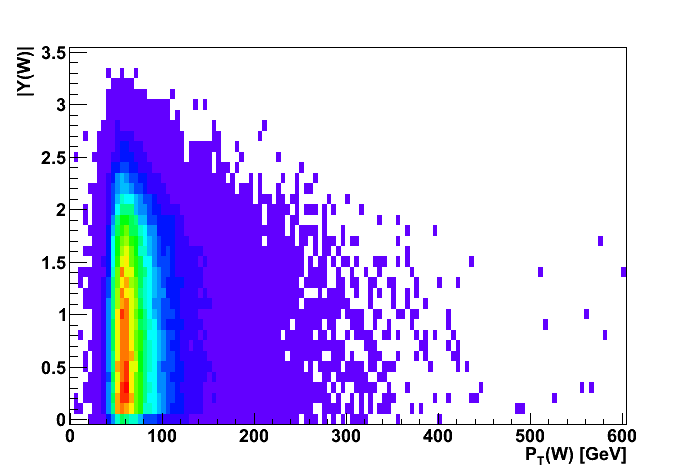
\includegraphics[width=0.45\textwidth]{fig/WPTvsY_mcreco50toinf}}\quad
\subfloat[]{\label{fig:wpol_genreco_ppt}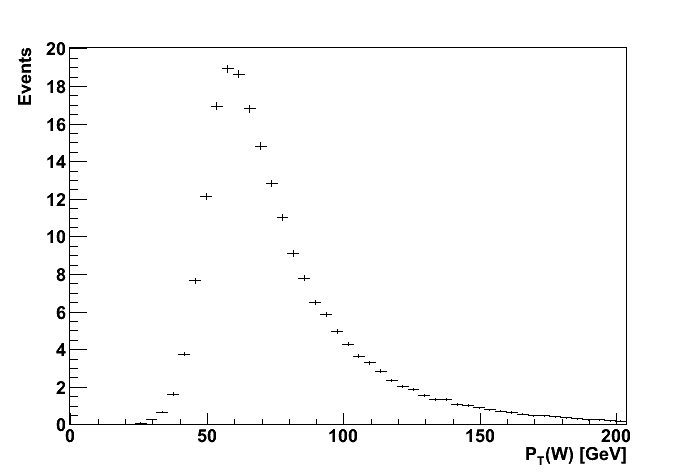
\includegraphics[width=0.45\textwidth]{fig/ptw_mcrecocut}}\quad
\caption{}
\label{fig:wpol_genreco}
\end{figure}

\subsubsection{Closure Test}
% Perhaps this section should be moved?
To ensure that the method is working correctly, several closure tests were
performed. Firstly, the generator-level helicity fractions within the phase
space of the reconstruction level \PW acceptance cuts are extracted. Essentially
the $\cos\thetastar$ distribution is plotted from a simulated sample of events
which have passed the reconstruction level \PtW cut. The distribution is fit,
once again using Eqn~\ref{eqn:wpol_helicity_fractions} and values of \f0, \fL and
\fR are extracted for both boson charges. This defines the baseline expectation
for the helicity fractions and is shown in Table~\ref{tbl:wpol_closure_tests}.

The first closure test has been performed in the muon channel only. The
generator level \LP templates for each helicity state are generated using the
re-weighting method as described in Section~\ref{sec:wpol_reweighting} but excluding
the acceptance correction. The phase space again corresponds to the
reconstruction levels cut on \PtW. The binned maximum likelihood fit is then
performed (see Section~\ref{sec:wpol_fitting}) and the helicity parameters
obtained are shown in Table~\ref{tbl:wpol_closure_tests}. The agreement with the
aforementioned generator level values is seen to be within the statistical error
of the simulated sample.

Finally, a full reconstruction level closure test was performed in both electron
and muon channels and applying all of the analysis cuts listed in
Section~\ref{sec:wpol_cutflow}. The results are also shown in
Table~\ref{tbl:wpol_closure_tests}. The muon channel is seen to recover the
``true'' helicity fractions to within their statistical error. The electron
channel, further complicated by \ac{QCD} contributions is seen to close within
the statistical error derived from the maximum likelihood fit. This corresponds
to \unit{100}{\invpicobarn} of simulated data.

\ctable[
cap=\PW Polarisation fit results for a number of closure tests,
caption=Fit results for the helicity fractions\, $f_{L}^{\pm}$ and $f_{R}^{\pm}$\,
for several closure tests of the re-weighting method described in
\sec~\ref{sec:wpol_reweighting}. The results of an analytical fit to the
$\cos\thetastar$ distribution\, having applied reconstruction level cuts on the
\PW boson\, are shown in the first column. The second column shows results from fits to the
\LP distribution at generator level in the muon channel. The final two columns
show the results of a full\, reconstruction-level closure test in both lepton
channels. The uncertainties have not been included for the reconstruction-level
muon fit since it is seen to close within the uncertanties of the analytical
fit.,
pos=h,
label=tbl:wpol_closure_tests,
doinside=\scriptsize
]{lcccc}{
}{\FL
            & Analytical Fit & Template Fit: Generator-Level & \Pgm Reconstruction-Level  & \Pe Reconstruction-Level \ML
$f_{L}^{-}$  & $0.5138 \pm 0.0032$     & 0.5149 & 0.5169 & $0.519\pm 0.038$\NN
$f_{R}^{-}$  & $0.2714 \pm 0.0027$     & 0.2708 & 0.2690 & $0.263\pm 0.040$\NN
$f_{L}^{+}$  & $0.5485 \pm 0.0026$     & 0.5506 & 0.5507 & $0.549\pm 0.048$\NN
$f_{R}^{+}$  & $0.2270 \pm 0.0021$     & 0.2286 & 0.2291 & $0.235\pm 0.019$\LL
}

\section{Analysis}
\subsection{Introduction}
To summarise what has already been said, the goal of this analysis is to extract
the helicity fractions (\fL, \fR and \f0) of the \PW boson and thus establish
the dominant left-handed polarisation effect present in theoretical predictions
at high \PtW. The $f_i$ coefficients determine the polar angle distribution
(\thetastar) via Eqn~\ref{eqn:wpol_helicity_fractions}. This distribution cannot
be reconstructed directly due to an ambiguity in the reconstruction of the \PW
boson rest frame. Instead the \LP variable, found to be highly correlated with
$\cos\thetastar$ in the limit of large \PtW is taken instead. Via a re-weighting
method, \LP distributions are constructed from Monte-Carlo simulation
corresponding to 100\% left-handed, right-handed and longitudinally polarised
\PW bosons. These shapes may then be used in a fit to data in order to extract
the helicity fractions themselves.

It should be noted that the $f_i$ coefficients are expected to differ between
\PWp and \PWm. However, they are not expected to depend on the flavour of the
decay lepton. This is relevant to two aspects of this analysis. Firstly, as
shall be seen, the $\PW\longrightarrow\Ptau\Pgn$ decays where the \Ptau decays
to either and electron or a muon are included in the dataset. Secondly,
information from both electron and muon channels may be combined to constrain
the helicity fractions.

In order to perform this analysis, it is vital that a highly pure sample of \PW
bosons is collected. Additional background contamination must be accounted for
in the fitting procedure, either by subtraction or by incorporation of an
appropriate shape template. However this is handled, it will inevitably
introduce additional uncertainty into the fit. In the case of subtraction,
uncertainty on the shape and normalisation must be accounted for and propagated
into the total uncertainties on the helicity fractions. Introducing an
appropriate template into the fit adds an additional parameter to account for
the relative normalisation as well as uncertainties stemming from the template
shape. This is particularly problematic in the case of \ac{QCD} multi-jet events
where the underlying processes are felt to be poorly understood. This
necessitates the use of a data-driven template which, as will be seen, brings an
additional set of difficulties.

\subsection{Backgrounds}
\label{sec:wpol_backgrounds}
It will be helpful to begin with a discussion of the backgrounds relevant to
this analysis. However, in order to understand the composition of the
backgrounds, the fundamental selection requirements should be stated. The
topology of interest are of course leptonic \PW decays, $\PW \longrightarrow
\Pl\Pgn$. In addition, the polarisation effect described in
Section~\ref{sec:polarisation} is associated with \PW bosons produced with a
large transverse momentum. As was previously described, this serves to enhance
the quark-gluon interactions which lead to a strong left-handed
polarisation. Therefore, we find that the two most essential selection
requirements are:
\begin{itemize}
\item A single isolated lepton typical of a \PW decay
\item An event topology consistent with a large transverse momentum \PW. As shall
  be seen in Section~\ref{sec:wpol_wpt}, there is some freedom in the exact
  variables used to achieve this selection.
\end{itemize}
Taking only these two requirements, a considerable background will remain. As
will be shown, this can be largely eliminated via additional selection
criteria. The principal background sources may be categorised as follows:
\begin{itemize}
\item Drell-Yan production leading to a dilepton final state in which one of the
  leptons is missed due to acceptance, poor reconstruction or other detector
  effects.
\item \ttbar production where $t\longrightarrow\Pbeauty\PW$ and the \PW then decays
  leptonically.
\item \ac{QCD} multi-jet events. This can be due to jet punch-through overlapping
  with a charged hadron or heavy-flavour decays. Electrons face a much higher
  background due primarily to photon conversions and overlap between charged
  hadrons and \Ppizero. The charged hadron leaves a track, whilst the \Ppizero
  decay leads to a shower of photons in the \ac{ECAL}.
\item For the electron channel only, there is an additional background from the
  conversion of promptly produced photons in \gammajets.
\end{itemize}

\subsection{Leptons}
The first selection requirement is to choose events with a charged lepton
consistent with that of a \PW decay. Such events should, at a minimum, contain
at least one reconstructed electron or muon. Wherever possible, the lepton
selection criteria adopted were those used for the \PW cross section analysis
\cite{cms_w_paper}. These requirements had been chosen to be as robust as
possible during the period of early data-taking at \ac{CMS}.

\subsubsection{Muons}
\label{sec:wpol_muons}
The requirements placed on the muon are as follows:
\begin{itemize}
\item The muon is required to be reconstructed as both a global muon and a
  tracker muon. This is to guard against either global muons mismatched with the
  tracker or noisy muon chambers in the case of tracker muons. For further
  information on muon identification, see Section~\ref{sec:reco_muons}.
\item More than 10 hits in the tracker.
\item Bad muon fits are rejected by requiring $\chi^2 < 10$ on the global muon
  fit (tracker and muon chambers)
\item The transverse impact parameter of the muon with respect to the beam-spot
  is required to be $ < \unit{2}{\milli\metre}$. This is a fairly loose
  requirement but still rejects the majority of cosmic muons.
\item At least 1 hit is required in the pixels of the tracker in order to remove
  in-flight decays.
\item The tracker muon reconstruction must involve at least 2 muon stations. This suppresses
  punch-through and accidental matchings and ensures compatibility with the
  trigger.
\item The global muon reconstruction must involve at least 1 valid hit in the
  muon chambers; again to guard against decays in flight and punch-through.
\item A cut on the muon pseudorapidity $|\eta| < 2.1$ in order to ensure
  compatibility with the trigger requirements.
\item A cut on the combined isolation,
\begin{equation}
\CombIso = \frac{\sum_{\textrm{tracks}} p_T^{\textrm{track}} + \sum_{\textrm{dep}}
  E_T^{\textrm{had}} + \sum_{\textrm{dep}} E_T^{\textrm{had}}}{\Ptmu} < 0.1
\label{eqn:wpol_mu_comb_iso}
\end{equation}
where the sums run over the tracks in the tracker or the energy deposits in the
\ac{ECAL} and \ac{HCAL} within a cone of $\Delta R = \sqrt{(\Delta\eta)^2 +
  (\Delta\phi)^2} < 0.3$. A threshold of \unit{0.7}{\GeV} was placed on the
tracks contributing to the isolation sum.
\end{itemize}
Muons passing this set of selection criteria will be referred to as
\textbf{Tight}. Global muons failing one or more of these criteria will be
referred to as \textbf{Loose}.

\subsubsection{Electrons}
\label{sec:wpol_electronid}
The electron identification variables used are as described in
Section~\ref{sec:reco_electron_id}. In order to achieve a strong suppression of
the \ac{QCD} multi-jet background, the decision was made to choose a tighter
working point than other \ac{CMS} analyses - the 70\% efficiency working
point. Electrons passing these criteria will be referred to as
\textbf{Tight}. For the purposes of vetoing dilepton events, the 95\% efficiency
cuts were used. These will be referred to as \textbf{Loose} electrons.

An additional requirement placed on the electron is that three distinct
measurements of the charge agree. This ensures that the charge misidentification
rate is suitably low for any resulting systematic uncertainty to be neglected
(see Section~\ref{sec:wpol_syst_charge_misid}).
% TODO more detail on the choice of the 70\% working point. Perhaps should be
% added later on.

\subsection{Jets}
\label{sec:wpol_jets}
In order to reject events coming from \ttbar decays, which tend to have a large
jet multiplicity, an upper limit is placed on the number of jets in the
event. The jets are clustered using the \antikT algorithm from particle flow
reconstructed objects. A cone radius of 0.5 is used and an acceptance cut
$\modeta < 5$ is applied.

Additionally, cleaning is applied to events in which a jet overlaps with the
leading lepton. These cases are assumed to result from some misreconstruction
and thus should be excluded from the analysis. In the case of the electron, the
nature of the reconstruction algorithms introduces many such
overlaps. Consequently, jets found to lie within a cone $\Delta R < 0.3$ of the
highest \Pt lepton in the event are simply removed from consideration. In
contrast, for the muon channel, a much tighter cut can be afforded. Events are
completely vetoed from the selection if a single jet is found to lie within a
cone $\Delta R < 0.5$ of the muon.

\subsection{Kinematic Cuts}
\subsubsection{Transverse \PW Momentum}
\label{sec:wpol_wpt}
The most vital kinematic cut to the analysis is the cut on the transverse
momentum of the \PW, \PtW. As has been discussed, requiring \PW bosons with a
large transverse momentum serves to enhance the polarisation effect described in
Section~\ref{sec:polarisation}. It also ensures the correlation of \LP with
$\cos\thetastar$ and thus improves the measurement of the helicity
fractions. There are several means of reconstructing the \PtW at \ac{CMS}. The
first, which was initially used for this analysis was the hadronic recoil of the
event. This is effectively the so-called missing hadronic energy of the
event, or \MHT,
% TODO Perhaps this should be moved somewhere else?
\begin{equation}
\PtW^{\textrm{had}} = - \sum_{j \in \textrm{jets}} \vec{j}
\end{equation}
where the $j$ is taken to run over some subset of the jets in the event as
defined in Section~\ref{sec:wpol_jets} with some minimum transverse momentum
requirement. The sum is taken to denote a vectorial sum. Since the \PW and the
jets must balance in the lab frame, this in principal provides an accurate
measurement of \PtW. However, the reconstruction of the jets is difficult and
subject to uncertainties in the jet energy scale. A higher resolution
measurement can be achieved by utilising instead the \MET (effectively the
neutrino) and the lepton in the event. This leads to the definition,
\begin{equation}
\PtW^{\textrm{lep}} = \vec{\Pl} + \vec{\MET}
\end{equation}
This provides a higher resolution measurement of \PtW, as can be seen in
Figure~TODO. It is thus the variable adopted in this analysis.

A second question, is then the choice of the minimum cut value to place on
\PtW. On the one hand, increasing this cuts reduces the statistics of the
sample. A related difficulty for this analysis was the small size of the
simulated $\PW\longrightarrow\Pl\Pgn$ sample, particularly at higher \PtW. On
the other hand, the enhancement of the polarisation effect and the increased
correlation between $\cos\thetastar$ motivate a larger cut value. The benefits of
these two effects could also be gained by binning the sample in \PtW and
performing independent fits within each bin. Unfortunately, the data sample
available had inadequate statistics to make such an approach feasible. Instead,
a moderately large cut $\PtW > \unit{50}{\GeV}$ was adopted.
% TODO more detail on this choice!

\subsubsection{Missing Transverse Energy}
In terms of rejecting backgrounds, tightening object definitions can only
achieve so much. Additional rejection power can be gained via additional
kinematic cuts on the event topology. As has already been stated, the \ac{QCD}
multi-jet background is the most problematic due to the fact that it is
relatively poorly modelled by Monte Carlo event generators. The simplest way to
reject such events is via a missing energy type cut. \ac{QCD} multi-jet events do
not typically contain a source of genuine missing energy. Experimentally
observed \MET from these events is typically due to jet mismeasurements,
detector noise or other problems with the event reconstruction. In addition, for
the high \PtW events of interest to this analysis, the missing energy component
(i.e. the neutrino) is often quite large. A relatively moderate cut on the \MET
is therefore able to reject the majority of such \ac{QCD} events.

However, a cut applied directly on the \MET introduces an additional
problem. Specifically, the \MET cut is effectively a selection on the momentum
of the neutrino in \PW events. This removes events, where for instance the
lepton has taken the majority of the momentum from the \PW and the neutrino is
thus very soft. This of course alters the shape of the \LP distribution. Of
course, the template re-weighting method will account for this acceptance
effect via appropriate changes in the helicity templates. This change is shown
in Figure~TODO. However, as can be seen, the sculpting of the \LP distribution
serves to remove the differences between the left and right-handed template
shapes, thus increasing their correlation. This becomes problematic within the
fitting procedure, where the similar shapes naturally make the inference of the
helicity fractions more difficult.

For this reason, it is desirable to cut on a variable that is not intrinsically
correlated with either the charged or neutral lepton momentum. The transverse
mass, \MT, is one such variable. Transverse mass is a variable chosen to
approximate the invariant mass of a particle by using only transverse
quantities. It is defined as follows

\begin{equation}
\MT = \sqrt{2\Ptl\MET\left(1 - \cos\Delta\phi\left(\Ptl, \MET\right)\right)}
\end{equation}

The angular dependence (i.e. the $\cos\Delta\phi$ term) will effectively
compensate \PW decays in which either the charged or neutral lepton is soft
since these topologies will in general have a larger angular separation. Since a
momentum imbalance is exactly what is expected from the transverse polarisation
effect, the \MT cut avoids directly suppressing this effect.

Now considering the effect of the \MT cut on the background components, it is
not expected to strongly suppress either the \Zjets or \ttbar backgrounds since
these both contain real decays of a heavy particle. In the case of \ac{QCD}
multi-jet events, a balanced jet system has been badly reconstructed
such that one of the jets has been misidentified as a lepton. In general, the
fake \MET signature from these events will be small and thus rejected by the \MT
cut. In the case that the \MET component is larger due to a badly measured jet,
there are two possibilities:
\begin{itemize}
\item The mismeasurement has occurred on the jet that has been misidentified as a
  lepton. Since $\Delta\phi \sim 0$, the \MT cut should strongly suppress these
  events.
\item The mismeasurement has occurred on one of the other jets in the event. In
  this case, \MT may be large due to the large angular separation. Note however,
  that these events will in general be suppressed by the cut on \PtW
\end{itemize}

For the muon channel, it was found that a reasonably moderate cut $\MT >
\unit{30}{\GeV}$ was able to reduce the \ac{QCD} multi-jet background to
negligible levels. This was first demonstrated in simulation and then
cross-checked via comparison with genuine data. In the case of the electrons,
the background proved far more problematic. In the end, an $\MT >
\unit{50}{\GeV}$ cut was chosen for the sake of simplicity. For more detail on
the optimisation study in the electron channel, see
Section~\ref{sec:wpol_electron_opt}.

\subsection{Cut Flow}
\label{sec:wpol_cutflow}
Having discussed the selection requirements to be used in this analysis, the
actual cuts and cut values will now be presented. These are shown in
Table~\ref{tbl:wpol_cutflow}.

\ctable[
cap=Selection requirements for the \PW polarisation measurement,
caption=Selection requirements for the muon and electron channels in the \PW polarisation analysis,
pos=h,
label=tbl:wpol_cutflow,
doinside=\scriptsize
]{lcc}{
}{\FL
Selection             & Electron Channel & Muon Channel \ML
1 tight lepton        & $P_T^{\Pe} > \unit{25}{\GeV}$, $|\eta^{\Pe}| < 2.4$ & $P_T^{\Pgm} > \unit{15}{\GeV}$, $|\eta^{\Pgm}| < 2.1$ \ML
Veto 2nd loose electron or muon & $P_T^{\Pe} > \unit{15}{\GeV}$, $|\eta^{\Pe}| < 2.4$ & $P_T^{\Pgm} > \unit{10}{\GeV}$, $|\eta^{\Pgm}| < 2.1$\NN
 & $P_T^{\Pgm} > \unit{15}{\GeV}$ , $|\eta^{\Pgm}| < 2.1$ & $P_T^{\Pe} > \unit{15}{\GeV}$, $|\eta^{\Pe}| < 2.1$ \ML
$<4$ \ac{PF} jets & $\Pt > \unit{30}{\GeV}$, $|\eta| < 5.0$ & $\Pt > \unit{20}{\GeV}$, $|\eta| < 5.0$ \NN
Jet overlap veto & - & $\Delta R_{\textrm{min}}\left(\Pgm, \textrm{jet}\right) > 0.5$ \ML
\PW Boson \Pt & \multicolumn{2}{c}{$\PtW > \unit{50}{\GeV}$} \NN
\MT & $\MT > \unit{50}{\GeV}$ & $\MT > \unit{30}{\GeV}$ \LL
}

\subsection{Triggers}
During the 2010 data taking period, the \ac{LHC} instantaneous luminosity
continued to evolve rapidly. The increased luminosity necessitated tightening of
the various object trigger requirements in order to maintain a suitable rate for
offline storage. This required careful selection of triggers for the analysis in
order to maintain efficiency with respect to the offline cuts.

For the muon channel, the triggers evolved quite slowly. In general, the cleaner
muon signature makes the triggers less susceptible to pile-up effects. The
triggers used were as follows:
\begin{equation*}
\begin{cases}
\texttt{HLT\_Mu9}          & \textrm{run} < 147146 \\
\texttt{HLT\_Mu15\_v1} & \textrm{run} \geq 147146
\end{cases}
\end{equation*}
Where the number in the trigger name indicates the \Pt threshold applied to the
lepton. In contrast, the electron trigger thresholds evolved more rapidly,
\begin{equation*}
\begin{cases}
  \texttt{HLT\_Ele10\_LW\_L1R} & \textrm{run} < 140041 \\
  \texttt{HLT\_Ele15\_SW\_L1R} & 140041 \leq \textrm{run} < 143963 \\
  \texttt{HLT\_Ele15\_SW\_CaloEleId\_L1R} & 143963 \leq \textrm{run} < 146428 \\
  \texttt{HLT\_Ele17\_SW\_CaloEleId\_L1R} & 146428 \leq \textrm{run} < 147117 \\
  \texttt{HLT\_Ele17\_SW\_TightEleId\_L1R} & 147117 \leq \textrm{run} < 148819 \\
  \texttt{HLT\_Ele22\_SW\_TightEleId\_L1R\_v2} & \textrm{run} 148819 \leq \textrm{run} < 149181 \\
  \texttt{HLT\_Ele22\_SW\_TightEleId\_L1R\_v3} & \textrm{run} \geq 149181
\end{cases}
\end{equation*}
% https://twiki.cern.ch/twiki/bin/view/CMSPublic/SWGuideEgammaHLT
Where \texttt{EleX} indicates an electron with $p_T > \unit{X}{\GeV}$. The
\texttt{LW} and \texttt{SW} stand for large window and small window
respectively. Here, window refers to the electron pixel-matching window and thus
the large window cut is looser and intended to be used during start-up
conditions. All triggers include \HoverE cuts on the electron. In addition,
those with \texttt{CaloEleId} or \texttt{TightEleId} impose additional electron
identification requirements. The first applies only a \sigmaieta cut (see
Section~\ref{sec:wpol_electronid}), whilst the second applies constraints on the
angular matching variables between the track and the supercluster (\deltaphiin,
\deltaetain) in addition to the \texttt{CaloEleId} requirement.

\section{Monte Carlo Expectation}
\subsubsection{Simulated Samples}
For each background component listed in Section~\ref{sec:wpol_backgrounds}, an
appropriate simulated sample was used. In the case of the \Zjets, \ttbar and
\gammajets, the generator setup was as for the \Wjets sample - the \ac{MADGRAPH}
matrix element generator interfaced to \ac{PYTHIA}. In the case of the \ac{QCD}
background, a number of samples were used. In the case of the Muon channel, this
was a sample generated using \ac{PYTHIA} and binned in terms of the transverse
momentum of the hard interaction, \pthat. This ensures adequate statistics even
in the regions of high \pthat that will tend to pass the analysis selection.

For the electrons, still larger statistics were required in order to study the
\ac{QCD} background properties. For these, \ac{QCD} samples were further
enriched towards the analysis level selection by selecting generator-level
electrons, photons, charged pions and charged kaons passing a set of loose
generator-level identification cuts approximating the isolation quantities and
\HoverE. This is referred to as the \textbf{EMEnriched} sample. An additional
sample is enriched by similar means with decays from \Pbottom and \Pstrange
hadrons. This is referred to as \textbf{BCtoE}. Both samples are again produced
in \pthat bins as for the unenriched sample. This generator level enrichment is
intended to reduce the costs in terms of time and disk space in processing a
much larger number of events, the majority of which will be rejected by basic
analysis cuts. An unfortunate side effect of this enrichement is that the
variables used in the filtering procedure may no longer be studied in their full
range. This is an impediment to certain background estimation studies which can
choose to invert certain lepton identification cuts.

\subsection{Monte Carlo Signal and Background Expectations}
\label{sec:wpol_yields}
The expected event yields across the relevant simulated samples are shown in
Tables~\ref{tbl:wpol_electron_yields} and \ref{tbl:wpol_muon_yields} for
electrons and muons respectively. The component marked \ac{QCD} denotes the
unenriched sample in the case of the muons and the sum of the
\textbf{EMEnriched} and \textbf{BCtoE} in the case of the electrons.

\ctable[
cap=\ac{MC} event yields in the electron channel of the \PW polarisation analysis,
caption=\ac{MC} event yields in the electron channel after each of the
selection requirements listed in Table~\ref{tbl:wpol_cutflow}. The yields shown
correspond to \unit{1}{\invpb} of integrated luminosity. A measure of the signal significance\, $S/B$\, is also given.,
pos=h,
label=tbl:wpol_electron_yields
]{lcccccc}{
}{\FL
Cut                    & W+Jets & QCD     & Z+Jets & $\gamma$+jets & $t\bar{t}$ & $S/B$ \ML
Trigger                & 6887.0 & 621013  & 804.4  & 1664.1        & 85.7       & 0.0   \NN
%$== 1$ loose electron & 5606.8 & 18299.7 & 369.7  & 627.3         & 24.4       & 0.3   \\ \hline
$N_e = 1$             & 2819.7 & 214.6   & 170.7  & 64.4          & 14.0       & 6.1   \NN
$N_{\mu} = 0$         & 2819.6 & 214.5   & 169.9  & 64.4          & 12.1       & 6.1   \NN
$< 4$ jets             & 2816.2 & 213.5   & 169.2  & 64.4          & 6.7        & 6.2   \ML
W boson $P_{T} > 50$ GeV & 182.2 & 17.2 & 28.4 & 15.9 & 5.0 & 2.7 \NN
$M_T > 50$ GeV           & 122.8 & 2.7  & 3.7  & 3.1  & 3.3 & 9.6 \LL
}
\ctable[
cap=Event yields in the muon channel of the \PW polarisation analysis,
caption=Simulated event yields in the muon channel after each of the
selection requirements listed in Table~\ref{tbl:wpol_cutflow}. The yields shown
correspond to \unit{1}{\invpb} of integrated luminosity. A measure of the signal significance\, $S/B$\, is also given.,
pos=h,
label=tbl:wpol_muon_yields
]{lccccc}{
}{\FL
Cut                                         & $W+$Jets   & QCD                  & $Z+$Jets  & $t\bar{t}$ & $S/B$ \ML
%Cross-section (pb)                         & 31314 NNLO & $8.76 \times 10^{8}$ & 3100 NNLO & 157.5 NLO  & -     \\\hline\hline
Trigger                                     & 7033       & 493887               & 909       & 28.1       & 0.01  \NN
$N_{\mu}=1$, $N_{e}=0$                      & 5086       & 27792                & 376       & 11.4       & 0.18  \NN
$< 4$ jets                                  & 5067       & 27740                & 368       & 5.5        & 0.18  \NN
$\Delta R_{\textrm{min}}(\mu$, jet$) < 0.5$ & 4979       & 26762                & 358       & 5.3        & 0.18  \NN
Second Muon Veto                            & 4973       & 26762                & 232       & 4.3        & 0.19  \ML
$\PtW > \unit{50}{\GeV}$                    & 264        & 21.3                 & 14.6      & 3.1        & 6.8   \NN
$\MT > \unit{30}{\GeV}$                    & 218        & 0.0                  & 5.4       & 2.0        & 26.0  \LL
}

\section{Fitting Procedure}
\label{sec:wpol_fitting}
In order to extract the helicity fractions in
Eqn~\ref{eqn:wpol_helicity_fractions}, a binned maximum likelihood fitting
procedure is performed. This takes \LP shape templates from the three \PW
helicity states, a number of data-driven or Monte-Carlo estimated background
templates and extracts the most probably values of \fL, \fR and \f0 from the
data distribution. In order to test the procedure, this method is also applied
to Monte Carlo ``pseudodata'' to ensure that fitted helicity fractions match
those derived from the analytical fit (see Section~TODO) to within the quoted
errors. The fit itself is implemented in the \ac{RooFit} software framework,
which assists in constructing an appropriate likelihood function and performing
the necessary minimisation using the \ac{MINUIT} numerical optimisation code.

The number of signal events in a given histogram bin $i$ in terms of the
helicity fractions can be written as
\begin{equation}
S^j = \fL h_L^j + \fR h_R^j + (1-\fL-\fR)h_0^j
\end{equation}
where $h_i^j$ are each binned helicity templates derived from the reweighting
method described in Section~\ref{sec:wpol_reweighting}. The \f0
coefficient has been rewritten using the relation $\fL + \fR +\f0 = 1$ and thus
it is seen to be a two parameter fit.

As shown in Section~\ref{sec:wpol_yields}, a non-negligible background component
is present in both channels arising from Drell-Yan and \ttbar production. These
can be referred to collectively as electroweak background contamination. For
these processes, the simulation is believed to be accurate enough to include
simulated \LP shape templates directly in the fit. In addition, the ratio of the
\Wjets vs electroweak background contributions is fixed assuming \ac{NLO}
cross-sections. The combined electroweak background template is then
incorporated into the fit as follows:
\begin{equation}
E^j = f_{\textrm{sig}} S^j + (1-f_{\textrm{sig}}) B^j
\end{equation}
where $f_{\textrm{sig}}$ is the ratio of the \Wjets yield to the total simulated
yield and $B^j$ is the combined \LP template for the \Zjets and \ttbar
backgrounds. It should be emphasised that the variable $f_{\textrm{sig}}$ is not
free in the fit and thus does not introduce an additional degree of freedom.

The previous formula is adequate for modelling the muon channel. For the
electron channel, it has already been shown that \ac{QCD} multijet events as
well as \gammajets production provide a non-negligible additional
contribution. To deal with this, the formula is extended as follows:
\begin{equation}
N^j = (1 - f_{\textrm{qcd}}) E^j + f_{\textrm{qcd}}Q^j
\end{equation}
where $f_{\textrm{qcd}}$ is the ratio of the QCD multijet/\gammajets background
to the total event yield and $Q^j$ is a shape template derived via the procedure
described in Section~\ref{sec:wpol_data_driven_bg}. Unfortunately, as has
already been stated, the simulation of QCD events is not yet reliable for direct
inclusion into the fit - as for the electroweak backgrounds. From the
perspective of the fitting procedure, an important issue is that the relative
fraction $f_{\textrm{qcd}}$ cannot be predicted from simulation. It must either
be fixed by some data-driven measurement or allowed to float freely in the
fit. Whilst an independent measurement might perform better - given that \LP is
not designed to discriminate between electroweak and qcd backgrounds - it was
not possible on the timescale of this analysis. Instead, the value of
$f_{\textrm{qcd}}$ is allowed to float, introducing an extra degree of freedom
to the electron channel.

\subsection{Combined Fit}
It has been noted that the helicity fractions are charge dependent but lepton
flavour independent. This suggests that the measurement may be refined by
simultaneously fitting both muon and electron channels. Due to the lower
efficiencies in the electron channel, this is not quite a doubling of the
available statistics but should significantly reduce the statistical error. The
simultaneous fit multiplies the likelihood terms,
\begin{equation*}
\likelihood_{\textrm{sim}} = \likelihood_{\Pgm} \times \likelihood_{\Pe}
\end{equation*}


% TODO more on minimization here
% TODO
\section{Electron Channel}
\subsection{\ac{QCD} Background}
The principal difficulty faced by the electron channel over-and-above the muon
channel arises from the \ac{QCD} multijet background which, as has been seen,
remains even after tight kinematic and lepton identification cuts. This can be
discussed together with the promptly produced photon background (\gammajets)
which shares similar characteristics. These backgrounds enter the selection due
to some mismeasurement leading to a significant value of \PtW along with either
a real or fake lepton. They are highly problematic since their kinematics may
depend strongly on poorly understood \ac{QCD} processes - namely the production,
hadronisation and measurement of hadronic jets. Because of this, currently
available simulation codes cannot be fully relied upon to correctly model the
kinematics of these events. This is particularly true in the case of the \LP
variable which is sensitive to both the leptonic and missing energy components
of the event.

To solve the problem presented by \ac{QCD}, two approaches were taken. The
first, described in Section~\ref{sec:wpol_electron_opt} sought to suppress the
background as much as possible. This resulted in the tightened kinematic and
identification cuts that have already been detailed. The second focussed on
accurately modelling the remaining background component using a data-driven
procedure. This will be described in Section~\ref{sec:wpol_data_driven_bg}. It
should be noted that these two strategies do not always complement each
other. It was possible to achieve larger supression of the \ac{QCD} background
whilst worsening the fit result. This occurs because the data-driven template
becomes ``flatter'' and the fit is less able to distinguish it from the helicity
templates in the fit.

\subsection{Kinematics}
Before continuing, it is useful to discuss the appearance of the \ac{QCD}
background in terms of the \LP variable. To make this clear, consider the
measurement of \PtW via the hadronic recoil in a balanced multi-jet event where
a single jet has been misreconstructed as an electron. In this case, the
hadronic recoil will tend to point along the axis of the fake electron. If the
hadronic recoil is then used as a measurement of \PtW, it will be approximately
collinear with the \Pt of the fake electron and thus will yield a value of $\LP
\sim 1$. This can also be seen when the \PtW measurment is taken to be the
vector sum of \Ptl and \MET. The fake electron will tend to be poorly
reconstructed and thus collinear with the source of fake \MET, again leading to
$\LP \sim 1$. A similar argument can be made in the case of \gammajets events
where now the photon is the source of both fake \MET and the fake lepton.


\subsection{Cut Flow Optimisation}
\label{sec:wpol_electron_opt}with
A key challenge in the electron channel was posed by the significant background
from \ac{QCD} multijet events. The $\MT > \unit{30}{\GeV}$ cut applied in the
muon channel is unable to eliminate these events. An optimisation study was
undertaken to determine the optimal kinematic and lepton identification cuts,
quantified by the uncertainty obtained in the final template fit. Some
indication of the effect of the kinemtics cuts is given in
Figure~\ref{fig:wpol_ele_significance}. This shows the signal and background
yields as a function of varying \MET and \MT cuts applied after all other cuts
listed in Table~\ref{tbl:wpol_cutflow}. The background in this case is the sum
of the processes listed in Section~\ref{sec:wpol_backgrounds}. Also shown are
two possible measures of the signal significance, again with varying \MET and
\MT cuts. As can be seen, the \MET cut is significantly more effective at
supressing the background. However, this comes at the cost of considerably
reduced signal statistics. The significance plots could also be construed to
support a \MET cut over an \MT but of course, since the final results are
extracted from a template fit, the \LP shape must also be considered.

This point is further reinforced in Figure~\ref{fig:wpol_met_mt_fqcd}. Here the
$x$ and $y$ axes denote cut values of \MET and \MT. For each point on the plot,
the fraction of the total event yield due to \ac{QCD} mutlijet production is
plotted for those events surviving a combined cut on the \MET and \MT.

\begin{figure}
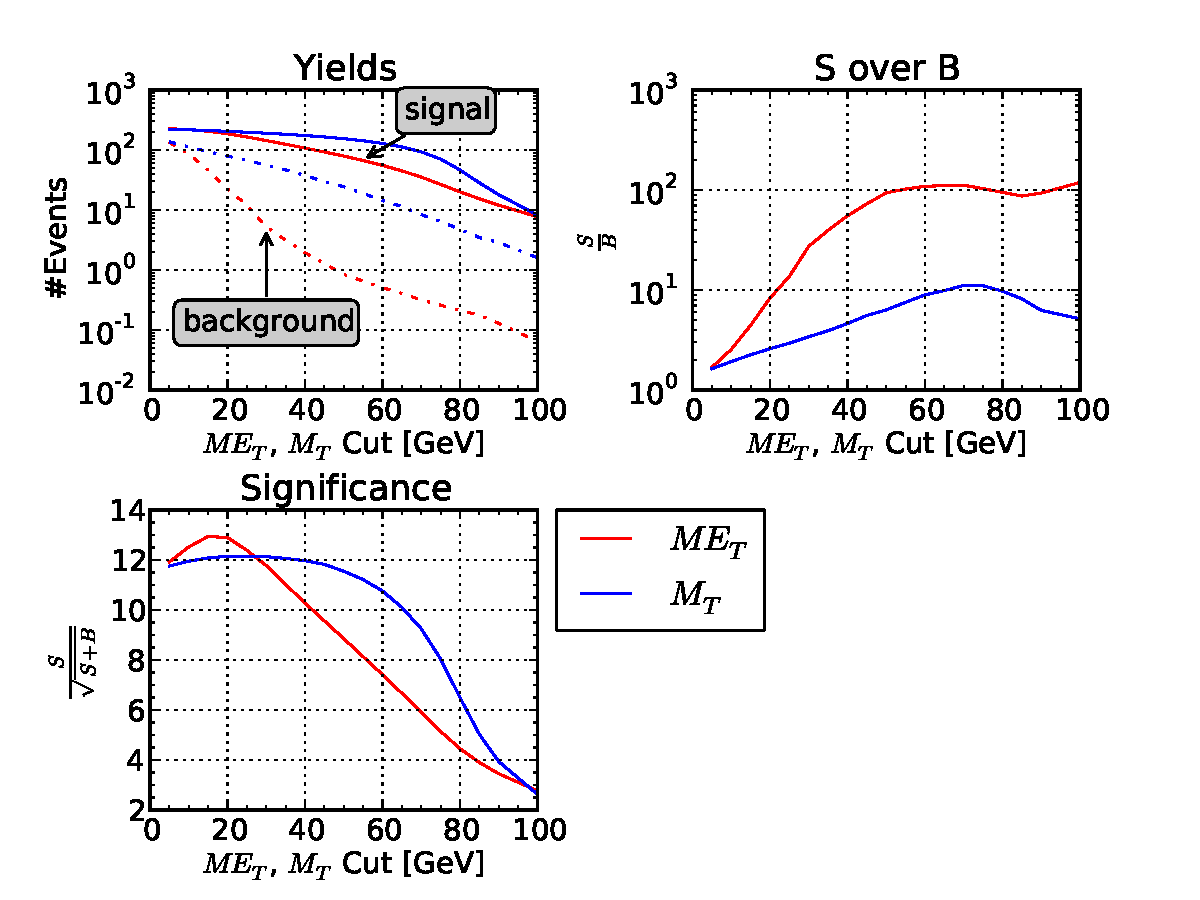
\includegraphics[width=0.8\textwidth]{fig/ewpol_significance}
\caption{Plot showing the significance of the electron channel TODO}
\label{fig:wpol_ele_significance}
\end{figure}

\begin{figure}
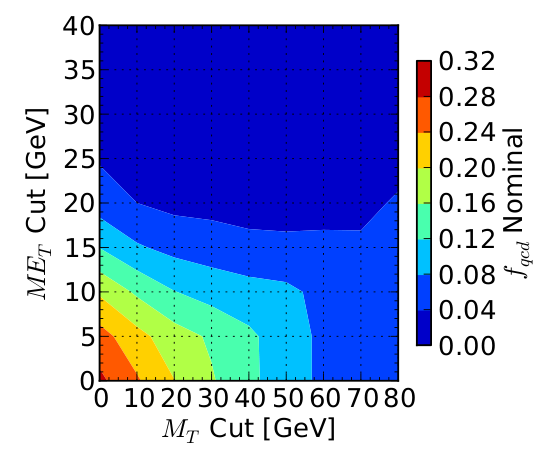
\includegraphics[width=0.7\textwidth]{fig/qcd_nom}
\caption{Plot showing the significance of the electron channel TODO}
\label{fig:wpol_met_mt_fqcd}
\end{figure}

The effect of a \MET or \MT $> \unit{30}{\GeV}$ cut on the shape of the \LP
templates for simulated \PWp events can be seen in
Figure~\ref{fig:wpol_met_vs_mt_templates}. The \ac{QCD} background is clearly
much reduced in the case of the \MET cut. However, as expected, the \MET cut
removes events with a soft neutrino. Put in a different way, these are events in
which the positron receives most of the energy from the \PW decay. The effect of
this is seen in the shape of the right-handed helicity templates, which has
clearly been cut away at $\LP \sim 1$.

\begin{figure}
\centering
\subfloat[]{\label{fig:wpol_met_vs_mt_templates_met}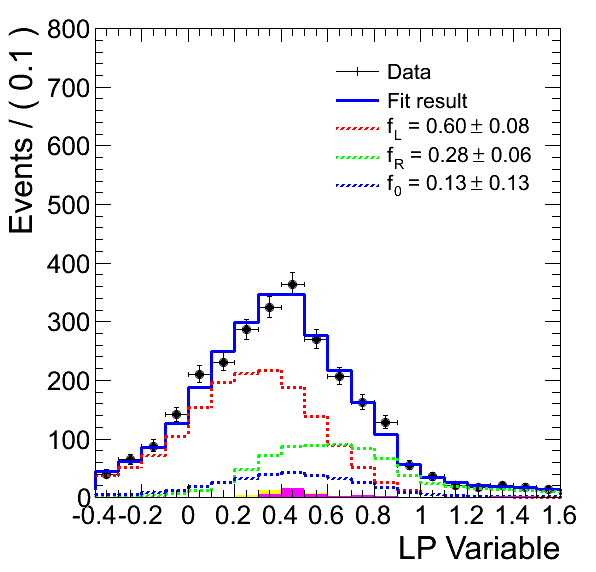
\includegraphics[width=0.4\textwidth]{fig/e_lp_fit_met30}}\quad
\subfloat[]{\label{fig:wpol_met_vs_mt_templates_mt}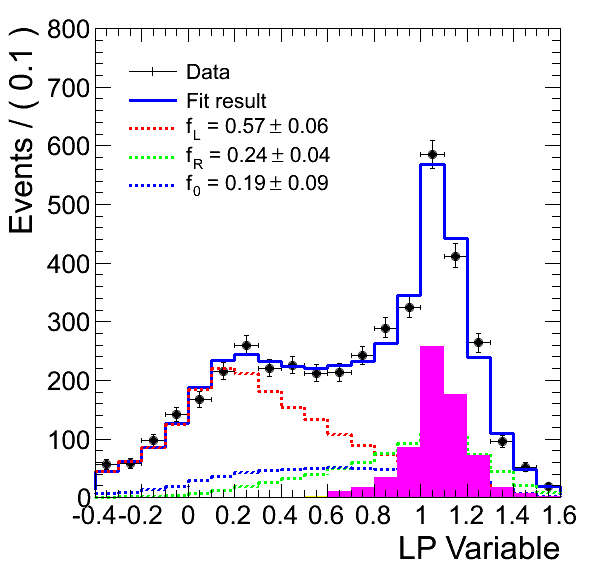
\includegraphics[width=0.4\textwidth]{fig/e_lp_fit_mt30}}
\caption[]{}
\label{fig:wpol_met_vs_mt_templates}
\end{figure}

\begin{figure}
\centering
\subfloat[]{\label{fig:wpol_wp80}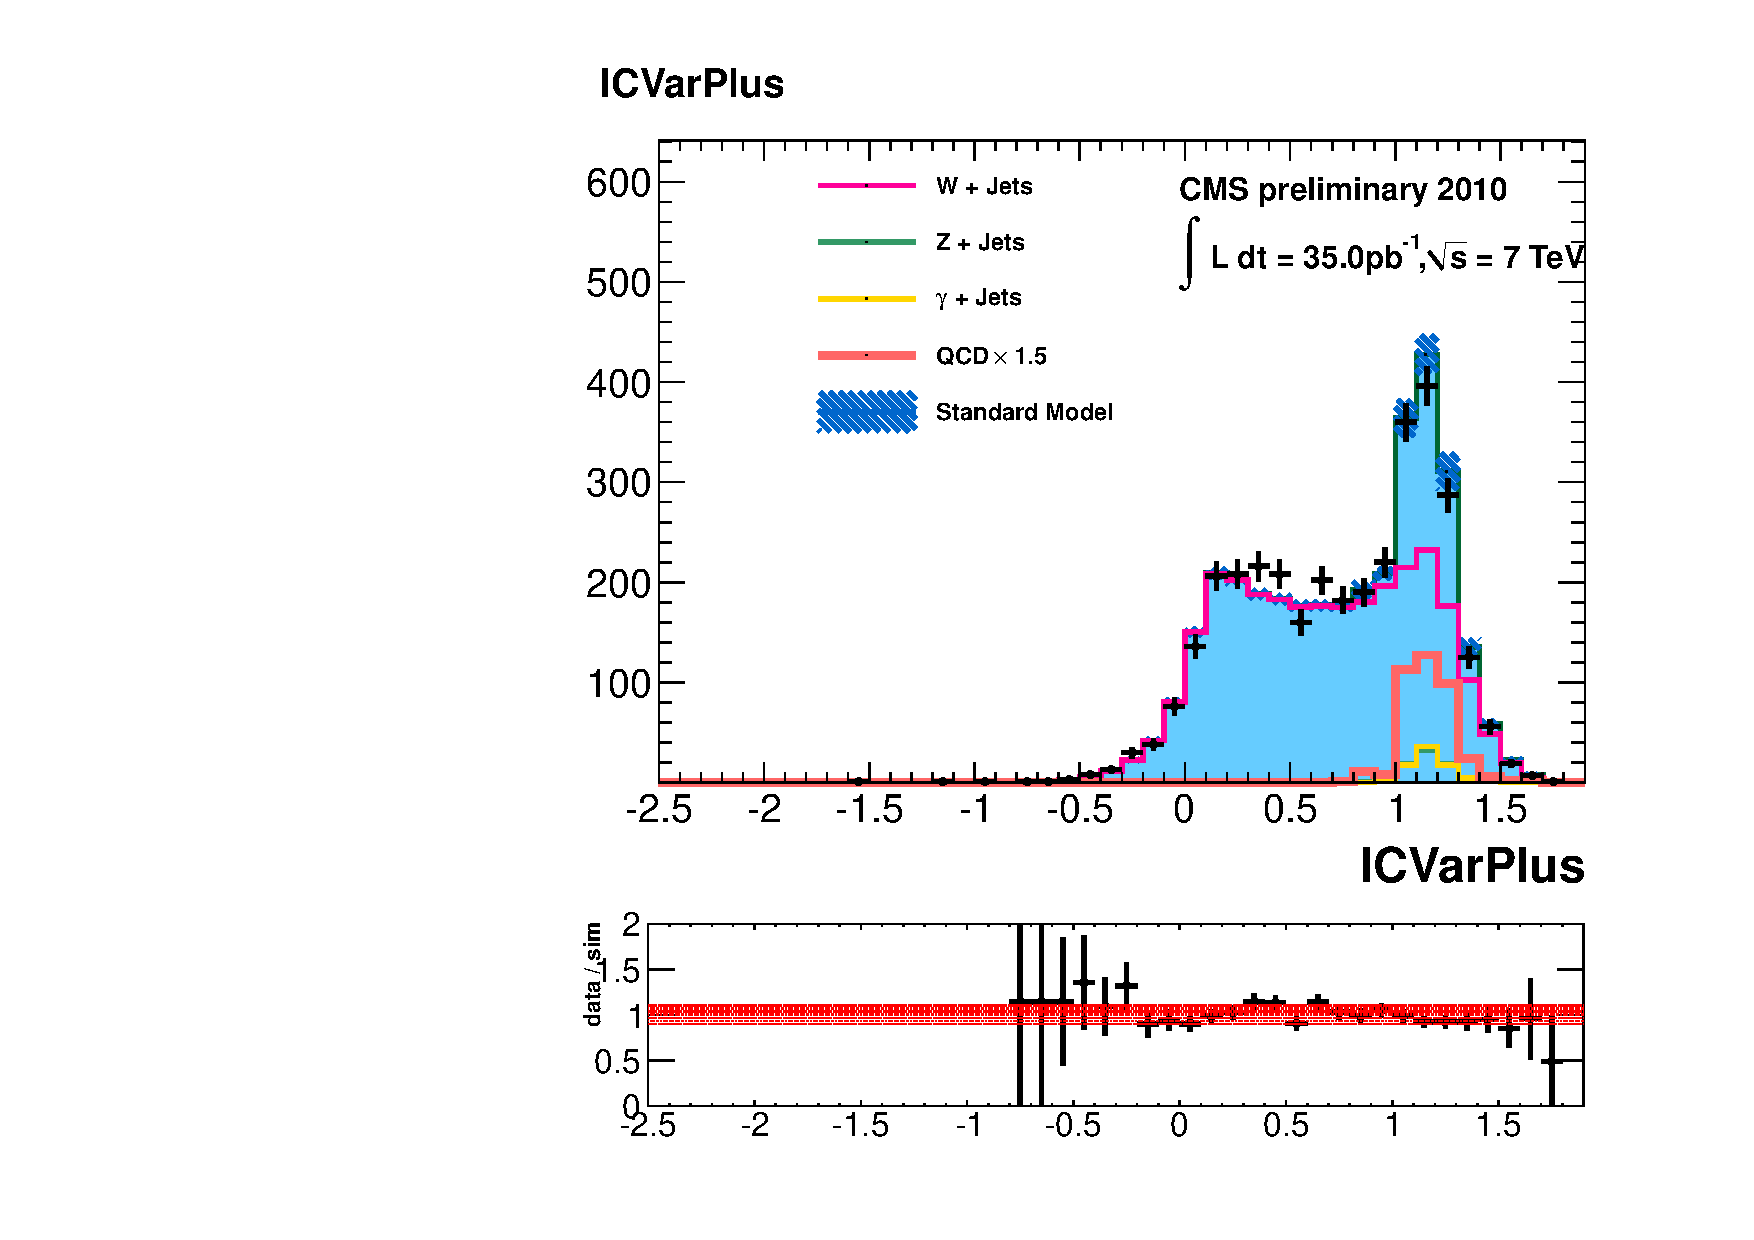
\includegraphics[width=0.4\textwidth]{fig/ICVarPlusMT50_WP80}}\quad
\subfloat[]{\label{fig:wpol_wp70}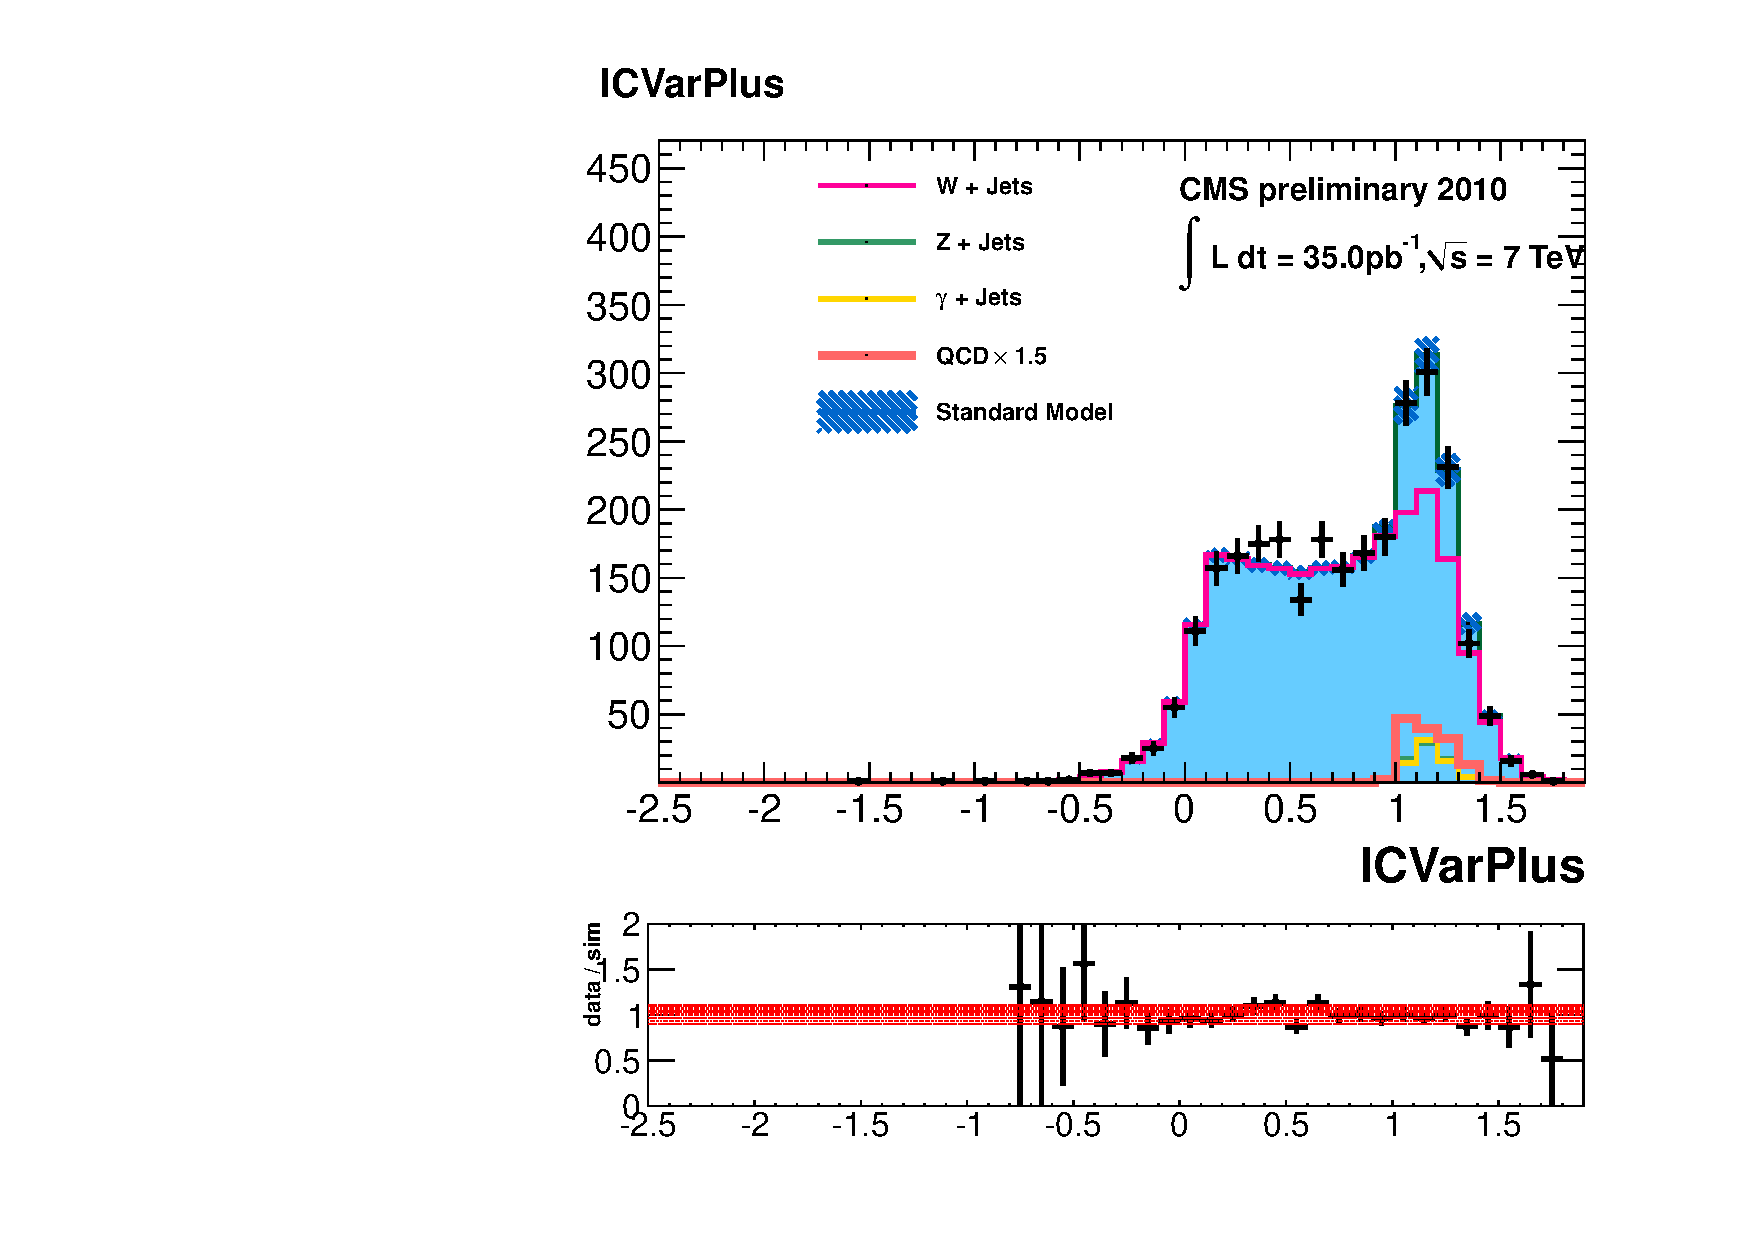
\includegraphics[width=0.4\textwidth]{fig/ICVarPlusMT50_WP70}}
\caption[]{The shape of the data \LP distribution and relevant backgrounds for
  two sets of electron ID cuts \subref{fig:wpol_wp80} WP80 and
  \subref{fig:wpol_wp70} WP70}
\label{fig:wpol_wp80_vs_wp70}
\end{figure}

\subsection{Data-Driven Background Template}
\label{sec:wpol_data_driven_bg}
To produce a reliable \LP shape template for \ac{QCD} and \gammajets events, a
data-driven procedure is needed which will yield a control sample enriched with
\ac{QCD} events resembling those entering the selected sample. Such a control
sample is often constructed by anti-selection. Consider the variables used for
the analysis selection as a multi-dimensional space in which the cut values
enclose some region which contains the selected sample - the ``selected''
region. The anti-selected sample is then constructed by inverting the cuts on a
subset of these variables. The region in this space selected by the inverted
cuts is then referred to as the ``anti-selected'' region. Since the majority of
the cuts are common to both selected and anti-selected samples, it can be
expected that they will share similar kinematic properties.

A variable suitable for inversion in this procedure must satisfy two
criteria. Firstly, it must provide separation power between the \ac{QCD}
background we wish to model and the other electroweak signal and background
events. Secondly, the \LP shape must be similar between the selected and
anti-selected regions. Put another way, the inverted variable must be
uncorrelated with \LP. An additional requirement is that the anti-selected
region (which may be the result of several inverted variables) contain adequate
statistics for construction of a shape template.

As the analysis was developed, a variety of anti-selection regions were tested
in simulation. One practical problem is that adequate statistics for these tests
could only be obtained by using the enriched \ac{QCD} sample. Since this sample
has an implicit cut on the electron isolation, it was not possible to study the
inversion of this variable. Many combinations of the electron identification
variables were tried. Many proved to be correlated with \LP via either the
leptonic or missing energy component.

In the end, the best compromise was achieved by inverting the track-supercluster
matching parameters, \deltaetain and \deltaphiin, on the leading electron. A
comparison of the selected and anti-selected shapes derived from this procedure
is shown in Figure~\ref{fig:wpol_ele_sel_antisel} before and after the \MT
cut. The \LP shape for \ac{QCD} background is not believed to have a charge
dependence and thus the shapes for positive and negative charge are combined
into a single template to mimimize statistical uncertainty.

\begin{figure}
\centering
\subfloat[]{\label{fig:wpol_antiselected1}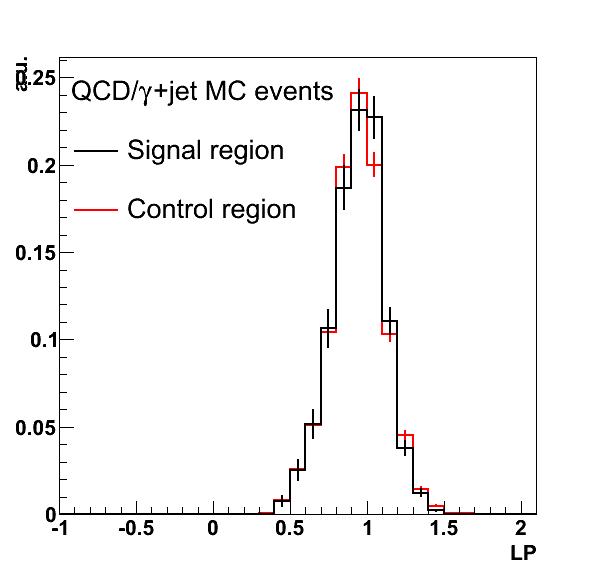
\includegraphics[width=0.4\textwidth]{fig/antiselected1}}\quad
\subfloat[]{\label{fig:wpol_antiselected2}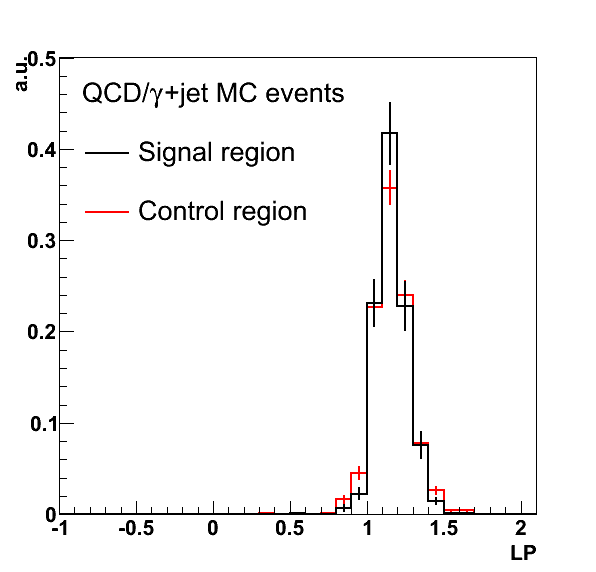
\includegraphics[width=0.4\textwidth]{fig/antiselected2}}
\caption[]{The \LP variable shown for selected (black) and anti-selected (red)
  simulated \ac{QCD} events after \subref{fig:wpol_antiselected1} $\PtW >
  \unit{50}{\GeV}$ and \subref{fig:wpol_antiselected2} $\MT > \unit{50}{\GeV}$}
\label{fig:wpol_ele_sel_antisel}
\end{figure}


\subsection{ECAL Transparency}

\section{Systematics}
\label{sec:wpol_systematics}
The template reweighting method necessary for the extraction of the helicity
fractions introduces an inescapable dependence on Monte Carlo simulation. One of
the challenges for this analysis is to ensure that any potential mismodelling
within the simulation which might affect the construction of the \LP templates
is properly accounted for and included as systematic uncertainties on the final
result. Such systematics may be broadly divided into experimental and
theoretical uncertainties.

\subsection{Experimental Uncertainties}
In considering the potential sources of systematic error, it is helpful to think
first in terms of the construction of the \LP variable. This involves two
detector level quantities: the missing transverse energy \MET and the transverse
momentum of the charged lepton \Ptl. The first quantity is derived from the
particle flow algorithm, as discussed in Section~TODO. The leading source of
uncertainty is due to the callibration of the jet energy scale.

\subsubsection{Jet Energy Scale}
\label{sec:wpol_syst_jec}
The jet energy scale is discussed in detail in Section~TODO. The uncertainty on
its callibration has been thoroughly studied and is parameterised as a function
of jet \Pt and $\eta$. In the case of a global miscallibration of this
measurement, jet energy measurements in data would be pushed upwards or
downwards with respect to the values predicted by simulation. If one imagines a
perfectly balanced dijet system in the centre of the detector, the resulting
effect on the \MET will of course be cancelled. However, this will rarely be the
case. In particular, in the case of \Wjets production, the hadronic system will
be recoiling against the \PW. For relatively high transverse momentum \PW
bosons, the \MET is very likely to point away from the recoiling jets. This
suggests that the effect of an upward or downard shift in the jet energy scale
is likely to have an opposite effect on the \MET scale and be highly correlated
betwen events. In other words, a shift in the jet energy scale will, to first
order, lead to an opposite shift in the \MET distribution. Of course there are
angular effects of an adjustment to the jet energy scale, which were fully
modelled in simulation. For now a heuristic argument will suffice to understand
the most striking effects.


The dominant effect of the jet energy scale on the fitted helicity fractions is
due to the change in the \LP shape. Of course, the effect will also affect the
cuts on \PtW and \MT and this has also been modelled in simulation. The shift in
the \MET due to the jet energy scale will correspond directly to a shift in the
calculated \LP. For an upwards shift in the jet energy scale, the \MET will tend
to shift downwards and thus to larger values of \LP. Conversely, for a downward
shift in the jet energy scale, the \MET scale will increase and therefore \LP
will shift to smaller values. This very approximate argument is born out in the
full modelling in simulation. This is illustrated in Figure~\ref{fig:wpol_mujecunc}
showing the fractional change of the \LP distribution in the muon channel for
upward and downward shifts in the jet energy scale. Clearly, the effect is quite
large and most severe towards the edges of the \LP distribution (i.e. $\LP < 0$
and $\LP > 1$). There are two reasons for this. Firstly, that in these regions
the \LP distribution is rising or falling rapidly. Bin to bin migration will
thus yield larger changes. Secondly, the change in the value of \LP for a single
event in response to a change in the jet energy scale is expected to be linear
in \LP to first order.

The jet energy scale is the dominant source of systematic uncertainty for both
electron and muon channels. The effect can be mitigated somewhat however by the
observation that a restricted fit range will insulate the measurement from the
most severe changes to the \LP shape. Whilst the edges of the \LP distribution
are the source of the largest jet energy scale uncertainty, they also tend to
contribute a lot to the fit. Reducing the fit range too drastically may remove
too much information from the fit, increasing the statistical error and negating
any benefits from the reduced systematic uncertainty. An optimisation study was
undertaken in both lepton channels and for both charges to choose an optimal fit
range.  The quadrature sum of the statistical and systematic errors was
calculated for a selection of possible fit ranges. It was determined that a fit
range of $[0,1.3]$ was an appropriate choice for both channels and both charges.

\begin{figure}
\centering
\subfloat[]{\label{fig:wpol_mujecunc_p}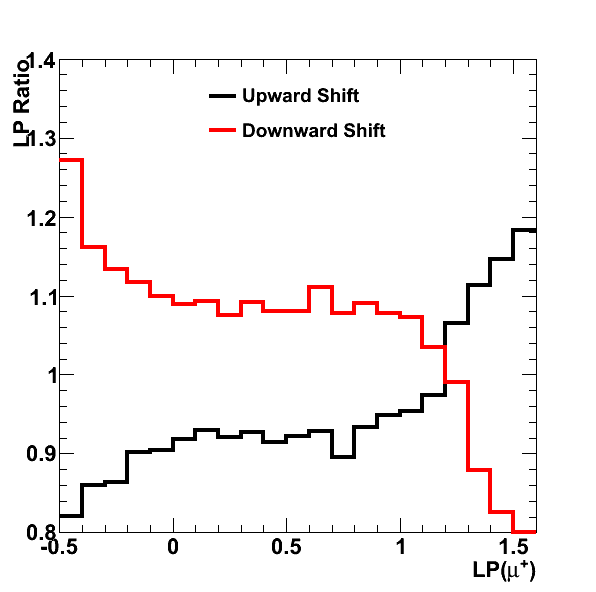
\includegraphics[width=0.4\textwidth]{fig/pLP_jecuncratios}}\quad
\subfloat[]{\label{fig:wpol_mujecunc_m}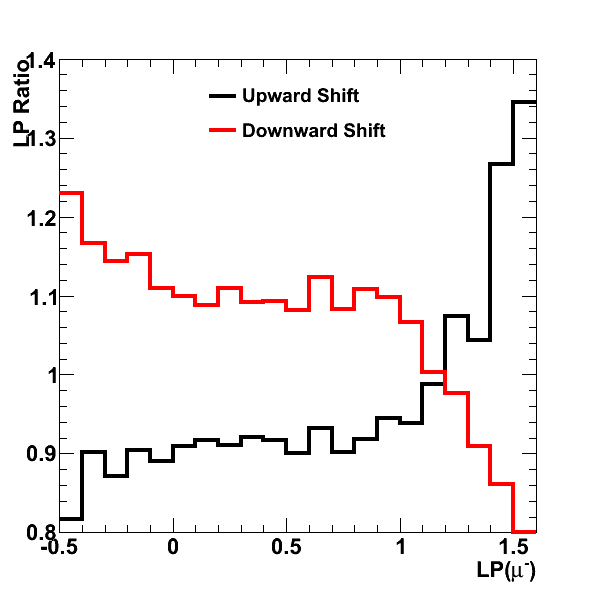
\includegraphics[width=0.4\textwidth]{fig/mLP_jecuncratios}}
\caption{}
\label{fig:wpol_mujecunc}
\end{figure}

The jet energy scale uncertainty follows the standard prescription for \ac{CMS}
analyses. Firstly, the unclustered component of the missing energy is calculated as,
\begin{equation}
\vec{E}^{\textrm{unclustered}}_T = -(\MET + \Ptl + \sum_i \vec{p}_T^{\textrm{jet},i}
\end{equation}
where the index $i$ runs over all jets with $\Pt > \unit{10}{\GeV}$ in the event
as reconstructed by the particle flow algorithm. The unclustered energy is then
scaled either up or down within its uncertainty (taken to be 5\%). The \MET is
then recalculated from this displaced unclustered energy,
\begin{equation}
\MET \longrightarrow -\vec{E}^{\textrm{unclustered}}_T - \Ptl - \sum_i (1 \pm  u(p_T, \eta)) \times \vec{p}_T^{\textrm{jet},i}
\end{equation}
where $u(p_T, \eta)$ is a map specifying the relative uncertainty on the jet
energy scale as a function of jet transverse momentum and pseudorapidity. The
scale applied to the jet momenta will be in the same direction as that of the
unclustered energy. When calculating the effect on the results, this displaced
value is then used in place of the \MET and all \MET derived quantities. The end
product of this are two modified \LP shapes corresponding to upward and downward
fluctuations in the jet energy scale. Since the shifted \MET has been applied
consistently throughout the analysis, the smaller effects on \PtW and \MT are
also included.

The value of the jet energy scale systematic is determined in simulation by
fitting the unaltered template (with no jet energy scale adjustment) to
pseudodata resulting from the upward and downward shifts. Taking the difference
of the upward and downward scaled cases with respect to the unaltered yields
asymmetric uncertainties on each of the helicity fractions. The final systematic
uncertainty is then taken to be largest of the two errors.

\subsubsection{\MET Resolution}
In addition to the modelling of the jet energy scale, another possible source of
mismeasurement stems from the resolution effects included in the simulation of
the detector. The resolution predicted by the Monte Carlo is believed to
considerably underestimate that observed in the data. To account for this,
additional ``smearing'' was applied to the missing transverse energy in
simulation. The difference between this ``increased resolution'' case and the
nominal conditions in simulation is then taken as an additional source of
systematic error.

As the first step of the procedure, the resolution on \PtW is extracted from the
simulation in bins of the generator level \PtW quantity. For simulated \Wjets
events with a reconstructed electron or muon and a matching generator level
particle or a generator level \Ptau, the following quantity is calculated,
\begin{equation}
\Delta\PtW = \frac{\left(\PtW\right)^{\textrm{GEN}} - \left ( \PtW \right)^{\textrm{RECO}}}{\left(\PtW\right)^{\textrm{GEN}}}
\end{equation}
This is the relative differnce between the reconstruction and generator level
\PtW. This distribution is then divided into bins of generator level \PtW. Each
bin is fit with a Gaussian distribution in order to extract the resolution as a
function of \PtW, $\sigma_{\PW}$. This is effectively the \PtW resolution as
modelled by the detector simulation.

The simulated sample is then used again, this time ``smearing'' the
reconstruction level \PtW quantity such that the resolution is increased by
10\%.

\subsubsection{Lepton Scale}
The second contribution to the \LP shape uncertainty comes from the lepton
momentum measurement. The character and magnitude of the uncertainty is quite
different between the electron and muon channels.

The muon momentum scale uncertainty due to material and B-field uncertainties
has been shown to be small. However, a charge asymmetric \Pt bias might appear
via ``$\chi^2$ invariant modes''. By calculating the difference in the \PZ mass
between events with a positive and negatively charged leading muon (in terms of
\Pt), the size of this effect can be judged. No significant effect is observed
in data. The errors on this measurement are used to place an upper bound on such
an effect. The effect is found to be less than 1\% at a \Ptmu of
\unit{100}{\GeV} and this is taken as a systematic uncertainty. This is
propagated to the helicity fractions by adjusting the \Ptmu in simulation by
$\pm 1\%$ and taking the difference from the unaltered case.

As described in Section~\ref{sec:reco_ecal_transparency}, the electron momentum is
corrected using continuous measurements of the \ac{ECAL} crystal
transparency. Unfortunately, these were not fully validated on the timescale of
this analysis (they were ready in the \ac{CMSSW} software version 3.9). Instead,
an alternative set of corrections were used, derived globally for the
dataset. This naturally has implications for the electron energy resolution,
since applying these global corrections per-event will widen the monetum
distribution while correcting the mean.

The transparency corrections were derived for the \PW charge asymmetry
measurement TODO. The detector is divided into 6 $\eta$ bins. The \Zee mass
distribution in data is then divided into $6 + ^6C_2$ categories corresponding
to cases where a \PZ is reconstructed from electrons in $\eta$ bins $i$ and $j$.
For each category a mass template is derived from simulation. A simultaneous fit
is then performed over the 21 categories, where each template is scaled by the
factor $1/\sqrt{s_is_j}$ and smeared by a resolution term $\sqrt{\sigma_i^2 +
  \sigma_j^2}$. The end result of this is a set of 6 scale terms and 6
resolution terms. These are plotted in Figure~\ref{fig:wpol_ecal_transp_corr}.
The scale terms should be applied to data, whilst the resolution should be
applied in simulation.

\begin{figure}
\centering
\subfloat[]{\label{fig:wpol_ecal_transp_scale}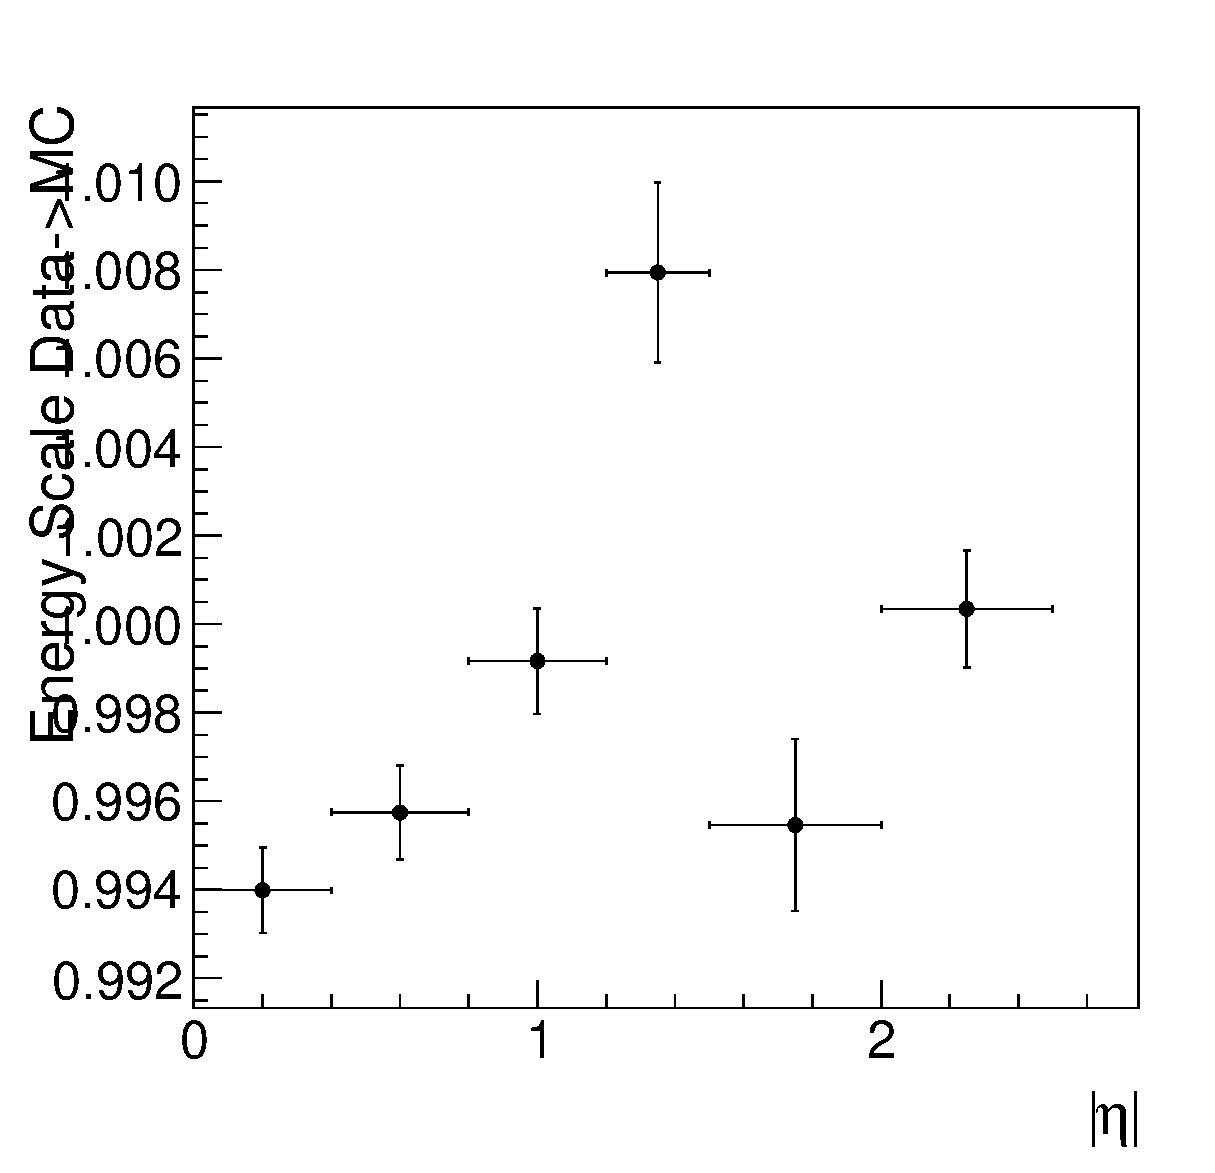
\includegraphics[width=0.45\textwidth]{fig/ecal_transp_scale}}\quad
\subfloat[]{\label{fig:wpol_ecal_transp_sigma}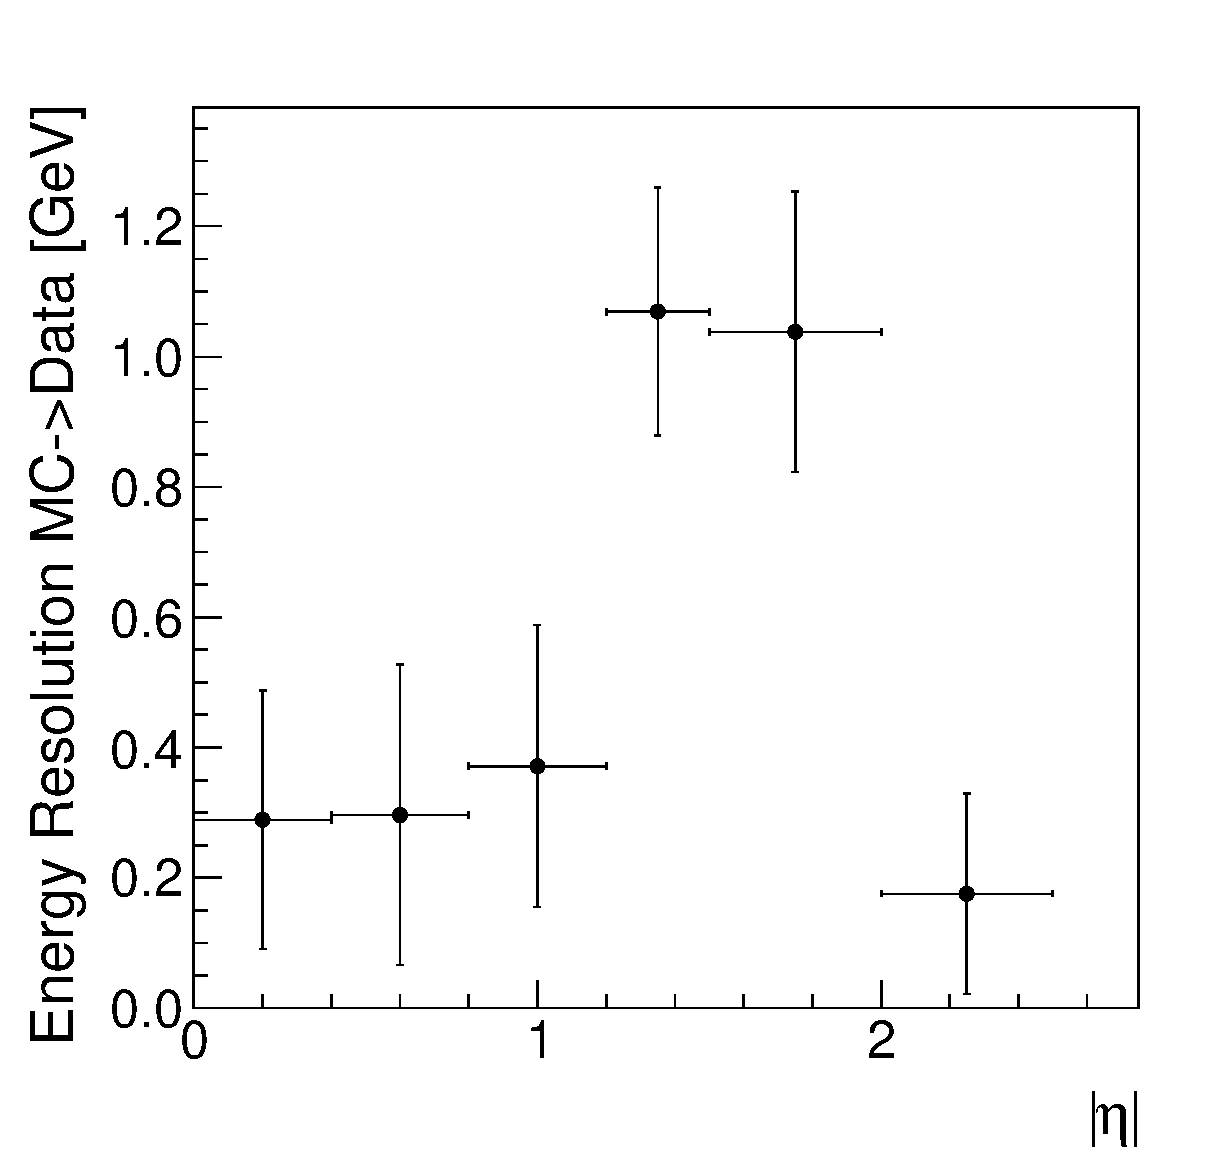
\includegraphics[width=0.45\textwidth]{fig/ecal_transp_sigma}}\quad
\caption[]{\ac{ECAL} transparency correction factors for
  \subref{fig:wpol_ecal_transp_scale} scale and
  \subref{fig:wpol_ecal_transp_sigma} resolution.}
\label{fig:wpol_ecal_transp_corr}
\end{figure}


The scale corrections have been applied in data. An conservative 50\%
uncertainty was taken on the value of the correction factors. The lepton
momentum in simulation is then adjusted by $\pm 50\%$ of the correction factor
and the resulting change in the fit results with respect to the unaltered case
is taken as a systematic uncertainty. This is equivalent to correcting the data
by either 50\% of 150\% of the correction factors.

The effect of the resolution corrections on the fit results was also judged by
applying them in Monte Carlo. The resulting change was found to be negligible,
and thus these factors were not applied in data.

\subsubsection{Electron \ac{QCD} Background Estimation}
\label{sec:wpol_syst_ele_bgest}
As discussed in Section~\ref{sec:wpol_data_driven_bg}, the template used to fit
the \ac{QCD} multijet background component in the electron channel has been
derived from a data-driven method. As has been shown, the simulation shows a
very similar \LP shape between the selected and anti-selected samples. However,
the small differences that can be seen coupled with the very limited statistics
available in Monte Carlo, necessitate the inclusion of an additional systematic
uncertainty.

The first systematic represents the degree, as can be judged from the enriched
\ac{QCD} Monte Carlo sample, that the anti-selected template mismodels the \LP
shape of the \ac{QCD} events in the selected region. In other words, the bias
introduced by any correlation between \LP and the track-supercluster matching
variables, as far as can be judged in simulation. This is evaluated by
performing TODO toy experiments. For each toy experiment, the Monte Carlo
pseudodata is first fitted using the \ac{QCD} template taken directly from the
selected region. This represents the case, where the \ac{QCD} has been modelled
perfectly by the template. Then the pseudodata is refit using the anti-selected
template and including contamination from the other simulated samples. The
ensemble distributions of the fit parameters are then compared between the
``true'' case using the actual \ac{QCD} Monte Carlo shape and the
``data-driven'' case using the anti-selected template. The difference in the
means of the ensemble distributions for the parameters \f0 and \fLmfR is then
taken as a systematic uncertainty. This is performed separately for both
charges.

The second systematic represents the uncertainty introduced by the very limited
statistics available in the simulated \ac{QCD}/\gammajets samples. This was
evaluated by redicing the Monte Carlo anti-selected template 500 times. Each
rediced template is fitted along with the standard signal and electroweak
background templates to the pseudodata. The ensemble distributions of \f0 and
\fLmfR are then plotted and the \ac{RMS} widths taken to be the systematic
uncertainty due to limited statistics in the \ac{QCD} template.

\subsubsection{Vertex Multiplicity}
The pile-up situation at \ac{CMS} was evolving rapidly as the instantaneous
luminosity increased. Due to the long lead-time in the generation of simulated
samples, it was not feasible to produce samples with vertex multiplicity
distributions exactly matching those present in data. In order to correct the
simulation to match the data, the simulated and observed vertex distributions
were compared. The simulated samples were then reweighted to account for this
difference. A systematic uncertainty is assigned by allowing the reweighting
factors to vary within their statistical uncertainties. The uncertainty was
tested in the muon channel and found to be negligible.

\subsubsection{Charge Misidentification}
\label{sec:wpol_syst_charge_misid}
Misidentification of the reconstructed lepton charge causes events to migrate
between the \PWp and \PWm samples. Since the templates are different for each
charge, this could bias the results of the fit. Any possible effect in the muons
is known to be negligible. For the electrons, the three charge requirement
brings the charge misidentification rate below 1\%. At this level, the
systematic related to charge misidentification is negligible in comparison to
the other sources of uncertainty.


\subsection{Theoretical Uncertainties}
In addition to the experimental uncertainties, the method relies upon
theoretical assumptions which can alter the extracted helicity fractions.

\subsubsection{\Ai Dependence}
Measurement of \f0 and \fLmfR will depend on the values of the other \Ai
coefficients. This was tested in simulation by varying each parameter \Ai by
10\% of its value - an uncertainty derived from comparison of \ac{LO} and
\ac{NLO} calculations by the Blackhat collaboration. The value of \fLmfR is
found to have a very small dependence on the values of the other \Ai.

\subsubsection{\ac{PDF} Uncertainties}
This analysis used a \Wjets Monte Carlo sample, generated using the \ac{CTEQ6L1}
\ac{PDF} set. This is a set of 41 \ac{PDF} distributions. All results in this
analysis are calculated using the best fit value of this set. To determine the
uncertainty associated with this assumption, each alternative \ac{PDF} from the
set is selected and modelled in the Monte Carlo via a reweighting
procedure. From this, 40 separate \LP distributions are derived representing
pseudodata assuming an alternative \ac{PDF} from the set. Each distribution is
then fit using the standard set of templates. The associated uncertainty is then
taken to be the average fluctuation from the nominal fit value across the 40 set
of alternate \acp{PDF}. This is found to be negligible for all polarisation
parameters ($< 0.01\%$).

\subsubsection{\Zjets and \ttbar Backgrounds}
For the purposes of the fit, the cross-sections of the electroweak backgrounds
are fixed both relative to each other and also to the \Wjets sample. To account
for uncertainty in the cross-section and efficiencies, the \Zjets and \ttbar
contributions were varied by $\pm 25\%$ and $\pm 50\%$ respectively. The
uncertainty on the helicity fractions is then taken to be the largest resulting
fluctuation from the nominal fit value. This has been calculated for both lepton
channels.


\ctable[
  caption=The relative effects on the values of \f0 and \fLmfR in the muon channel for the uncertainties described. The absolute values are shown in brackets.,
  label=tbl:wpol_mu_syst,
  doinside=\scriptsize
]{ c  p{2.5cm}  p{2.7cm}  p{2.5cm}  p{2.7cm}}{
}{\FL
     Uncertainty                         & $\fLmfR^{-}$                 & $\f0^{-}$                            & $\fLmfR^{+}$                & $\f0^{+}$ \ML
     \ac{JES}                            & $\pm11$\% (0.029)              & $\pm56$\% (0.123)       & $\pm3$\% (0.011)   & $\pm42$\% (0.092) \NN
     \MET Resolution                     & $\pm4$\% (0.012)               & $\pm3$\% (0.006)        & $\pm4$\% (0.012)   & $\pm2$\% (0.004)                        \NN
     $P_T(\mu)$ bias: $\pm$1\%/100 GeV   & $\mp$0.8\% (0.002)             & $\mp$ 11\% (0.004)      & $\pm1.2$\% (0.004) & $\mp$16.0\% (0.036)                   \ML
     Quadratic sum                       & $\pm12$\% (0.031)              & $\pm56$\% (0.123)       & $\pm5$\% (0.017)   & $\pm45$\% (0.099) \LL
}
\ctable[
cap=Systematic uncertainties in the electron channel,
caption={Sources of systematic uncertainty and their effect on the translation
factor, $R_{CS}$, in the electron channel. The relative uncertainty on the estimated number of events in the
signal region, stemming from the limited yield in the control
region, is also listed.},
pos=ht,
label=tbl:susy_syst_electrons
]{lcccc}{
}{\FL
                                   & \multicolumn{4}{c}{  \STlep Range (GeV) }\ML
                                   & [150-250] & [250-350] & [350-450] & $>$ 450\ML
$R_{CS}$                           & 0.16      & 0.18      & 0.19      & 0.23\ML
%$\Delta N/N$ at 1.1~fb$^{-1}$ (\%) & 12        & 22        & 38        & 58\ML
Systematic Uncertainty (\%)        & 14        & 20        & 24        & 34 \ML
Control Region Stat.      (\%)     & 5         & 9         & 17        & 24\NN
MC Stat.       (\%)                & 1         & 10        & 7         & 8 \NN
\ac{JES} (Flat 5\%)(\%)            & 9         & 10        & 10        & 19 \NN
\MET Resolution (10\%) (\%)         & 2         & 2         & 5         & 7 \NN
W/\ttbar Ratio (\%)                & 6         & 7         & 6         & 10 \NN
\ttbar($\ell\ell$) (\%)            & 6         & 7         & 6         & 2\NN
W Polarization (\%)                & 1         & 1         & 2         & 3\NN
\ttbar Polarization (\%)           & 5         & 5         & 5         & 5 \LL
}
\ctable[
  caption=The relative effects on the values of $f_{0}$ and $(f_{L} - f_{R})$ in the combined fit for the uncertainties described. The absolute values are shown in brackets.,
  label=tbl:tbl:combined_syst,
  doinside=\scriptsize
]{ l c  c  c  c }{
}{\FL
                                & $(f_{L} - f_{R})^{-}$  & $f_{0}^{-}$           & $(f_{L} - f_{R})^{+}$      & $f_{0}^{+}$      \ML
    PF Recoil Scale             & $\pm13$\% (0.033)      & $\pm60$\% (0.133)     & $\pm5$\% (0.016)          & $\pm40$\%  (0.087) \NN
    PF Recoil Resolution        & $\pm14$\% (0.035)      & $\pm10$\% (0.023)     & $\pm8$\% (0.027)          & $\pm7$\% (0.015) \NN
    Electron Scale $\pm50$\%    & $\pm5$\% (0.013)       & $\mp5$\% (0.011)      & $\mp4$\% (0.012)          & $\pm4$\% (0.008) \NN
    Muon Scale $\pm 1\%/100$GeV & $\mp<1$\% (0.002)      & $\mp3$\% (0.007)      & $\pm<1$\% (0.003)         & $\mp4$\% (0.008) \ML
    Quadratic Sum               & $\pm20$\% (0.050)      & $\pm62$\% (0.136)     & $\pm11$\% (0.034)         & $\pm40$\% (0.089) \LL
}
\ctable[
  cap=Theoretical uncertainties in the \PW polarisation measurement,
  caption=The relative effects on the values of \f0 and \fLmfR from theoretical uncertainties. The absolute values are shown in brackets.,
  label=tbl:wpol_theory_syst,
  doinside=\scriptsize
]{ c c c c c }{
}{\FL
                                             & $\fLmfR^{-}$  & $\f0^{-}$            & $\fLmfR^{+}$  & $\f0^{+}$            \ML
      $A_{1} \pm (A_{1}\times 10\%)$         & $\pm$0.2\% (0.0005)    & $\mp$4.4\% (0.0094)    & $\pm$0.2\% (0.0006)    & $\mp$4.9\% (0.0105)    \NN
      $A_{2} \pm (A_{2}\times 10\%)$         & $\pm$1.3\% (0.0033)    & $\mp$3.8\% (0.0081)    & $\mp$0.5\% (0.0016)    & $\mp$3.9\% (0.0084)    \NN
      $A_{3} \pm (A_{3}\times 10\%)$         & $\mp$0.4\% (0.0010)    & $\pm<$0.1\% (0.0002)   & $\pm<$0.1\% (0.0003)   & $\pm<$0.1\% (0.0002)   \ML
      $A_{0} + (A_{0}\times 10\%)$          & $<$0.1\%               & +10.6\%                & $<$0.1\%               & +10.5\%                \NN
      $A_{4} + (A_{4}\times 10\%)$          & +9.7\%                 & $<$0.1\%               & +10.2\%                & $<$0.1\%               \ML
      Z changed by 25\% (muon)               & $<$0.5\% (0.0013)      & $<$0.5\% (0.0011)      & $<$0.5\% (0.0016)      & $<$0.5\% (0.0011)      \NN
      \ttbar changed by 50\% (muon)      & $<$0.1\% (0.0003)      & $<$0.1\% (0.0002)      & $<$0.1\% (0.0003)      & $<$0.1\% (0.0002)      \ML
      Quadratic sum (muon)                   & $\pm$1.47\% (0.0037)   & $\pm$5.84\% (0.0125)   & $\pm$0.75\% (0.0024)   & $\pm$6.28\% (0.0135)   \ML
      \PZ changed 25\% (electron)              & $<$1\% (0.0022)         & $<$1\% (0.0020)      & $<$0.2\% (0.0006)       & $<$0.5\% (0.0010)     \NN
      \ttbar changed by 50\% (electron)  & 1.6\% (0.0041)          & 2.1\% (0.0045)         & $<$0.2\% (0.0005)      & 0.9\% (0.0019)      \ML
      Quadratic sum (electron)               & $\pm$2.3\% (0.0058)     & $\pm$6.1\% (0.013)      & $\pm$0.61\% (0.0019)   & $\pm$6.2\% (0.0136) \LL
}
\section{Results}
\label{sec:wpol_results}
\subsection{Datasets}
For this analysis, the full \ac{CMS} 2010 dataset was used with an estimated
integrated luminosity of \unit{36}{\invpicobarn}. The centre of mass energy
was $\sqrt{s} = \unit{7}{\TeV}$.

\subsection{Fit Results}
The individual fits of the \Pep, \Pem, \Pgmp and \Pgmm channels to the 2010
dataset are shown in Figure~\ref{fig:wpol_fit_results}. The signal and
background templates are shown individually along with the fitted values of
\fLmfR and \f0. The full error contour plots in the $(\fLmfR, \f0)$ plane are
shown in Figures~\ref{fig:wpol_contour_ele} and \ref{fig:wpol_contour_mu} for
electrons and muons respectively. It is clear in both cases that the predominant
left-handed polarisation described in Section~\ref{sec:polarisation} has been
observed with a large significance.

\begin{figure}
\centering
\subfloat[]{\label{fig:wpol_fit_ele_plus}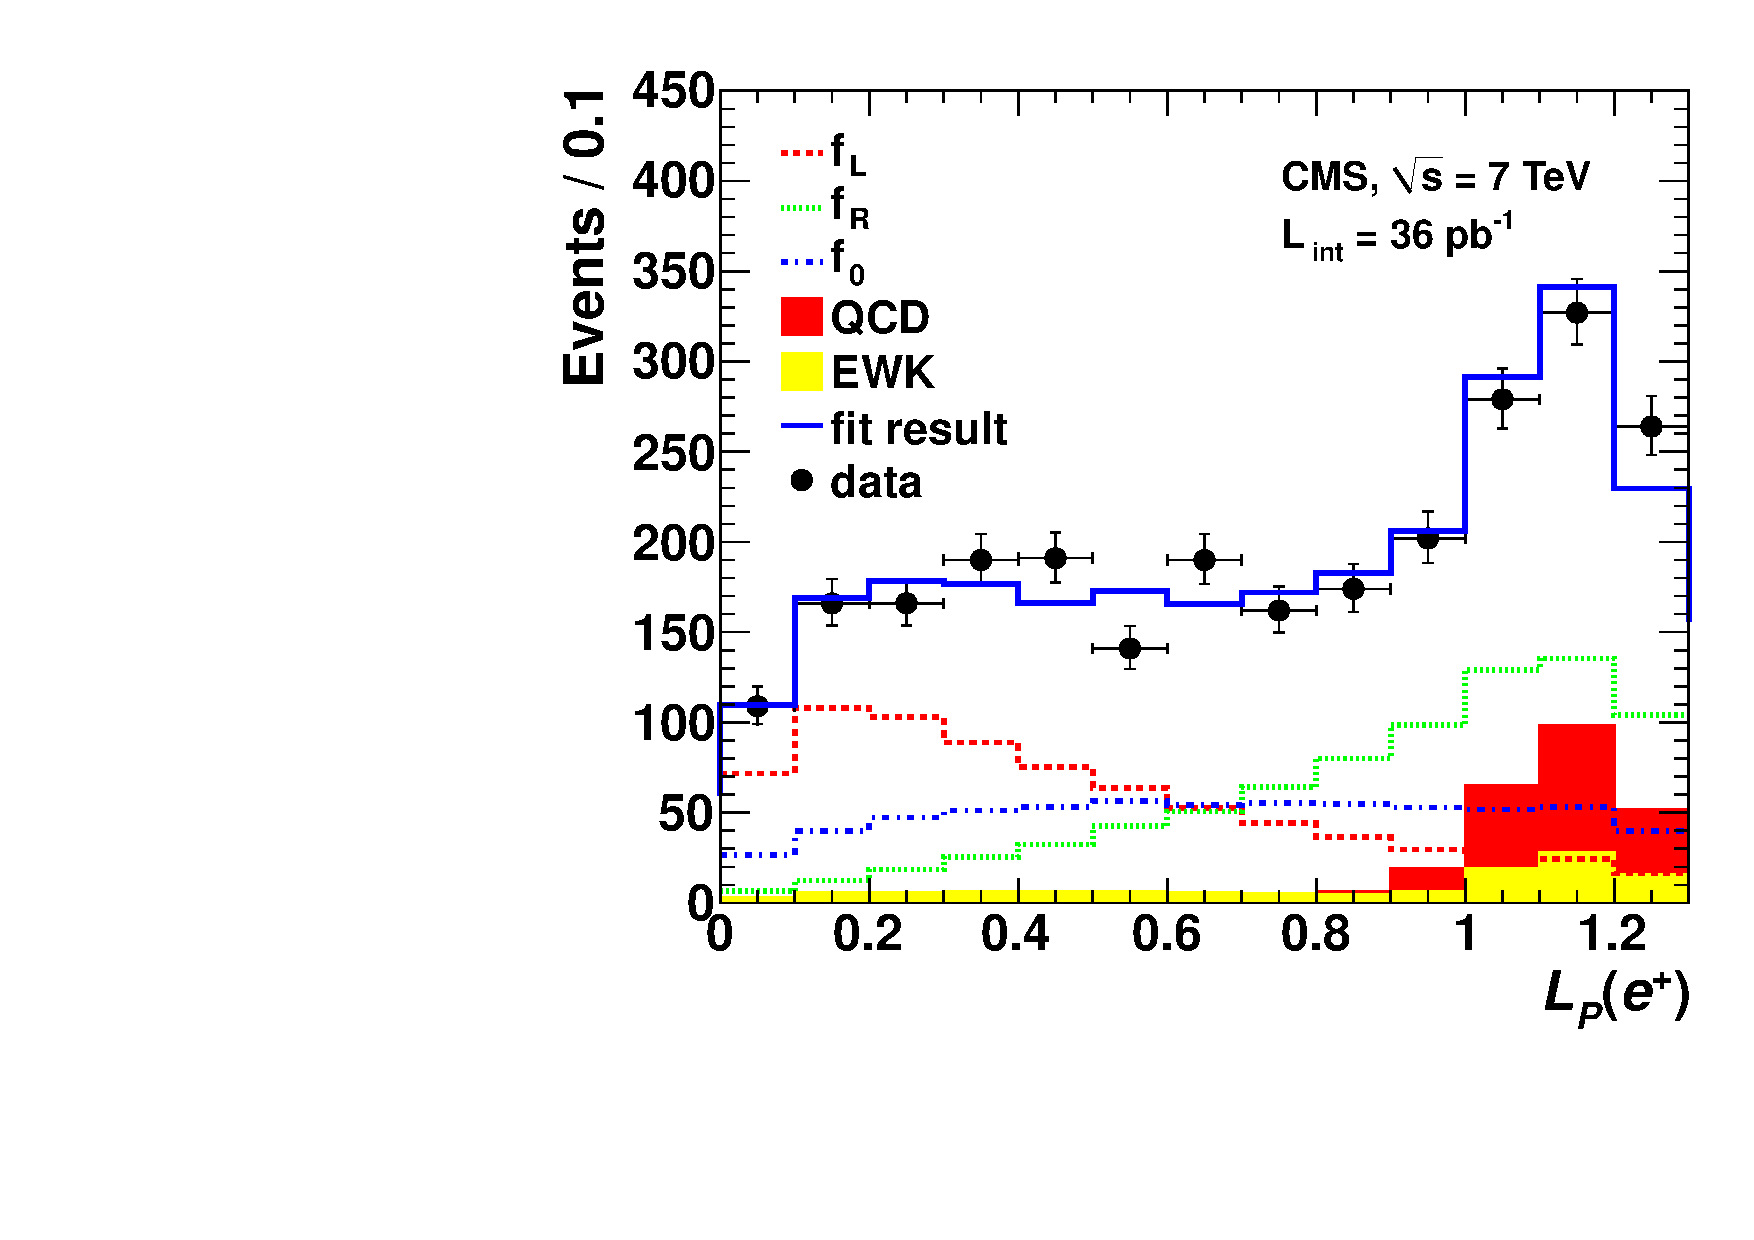
\includegraphics[width=0.45\textwidth]{fig/electron_MC_WHelicityFramePlots_PlusICVar}}\quad
\subfloat[]{\label{fig:wpol_fit_ele_minus}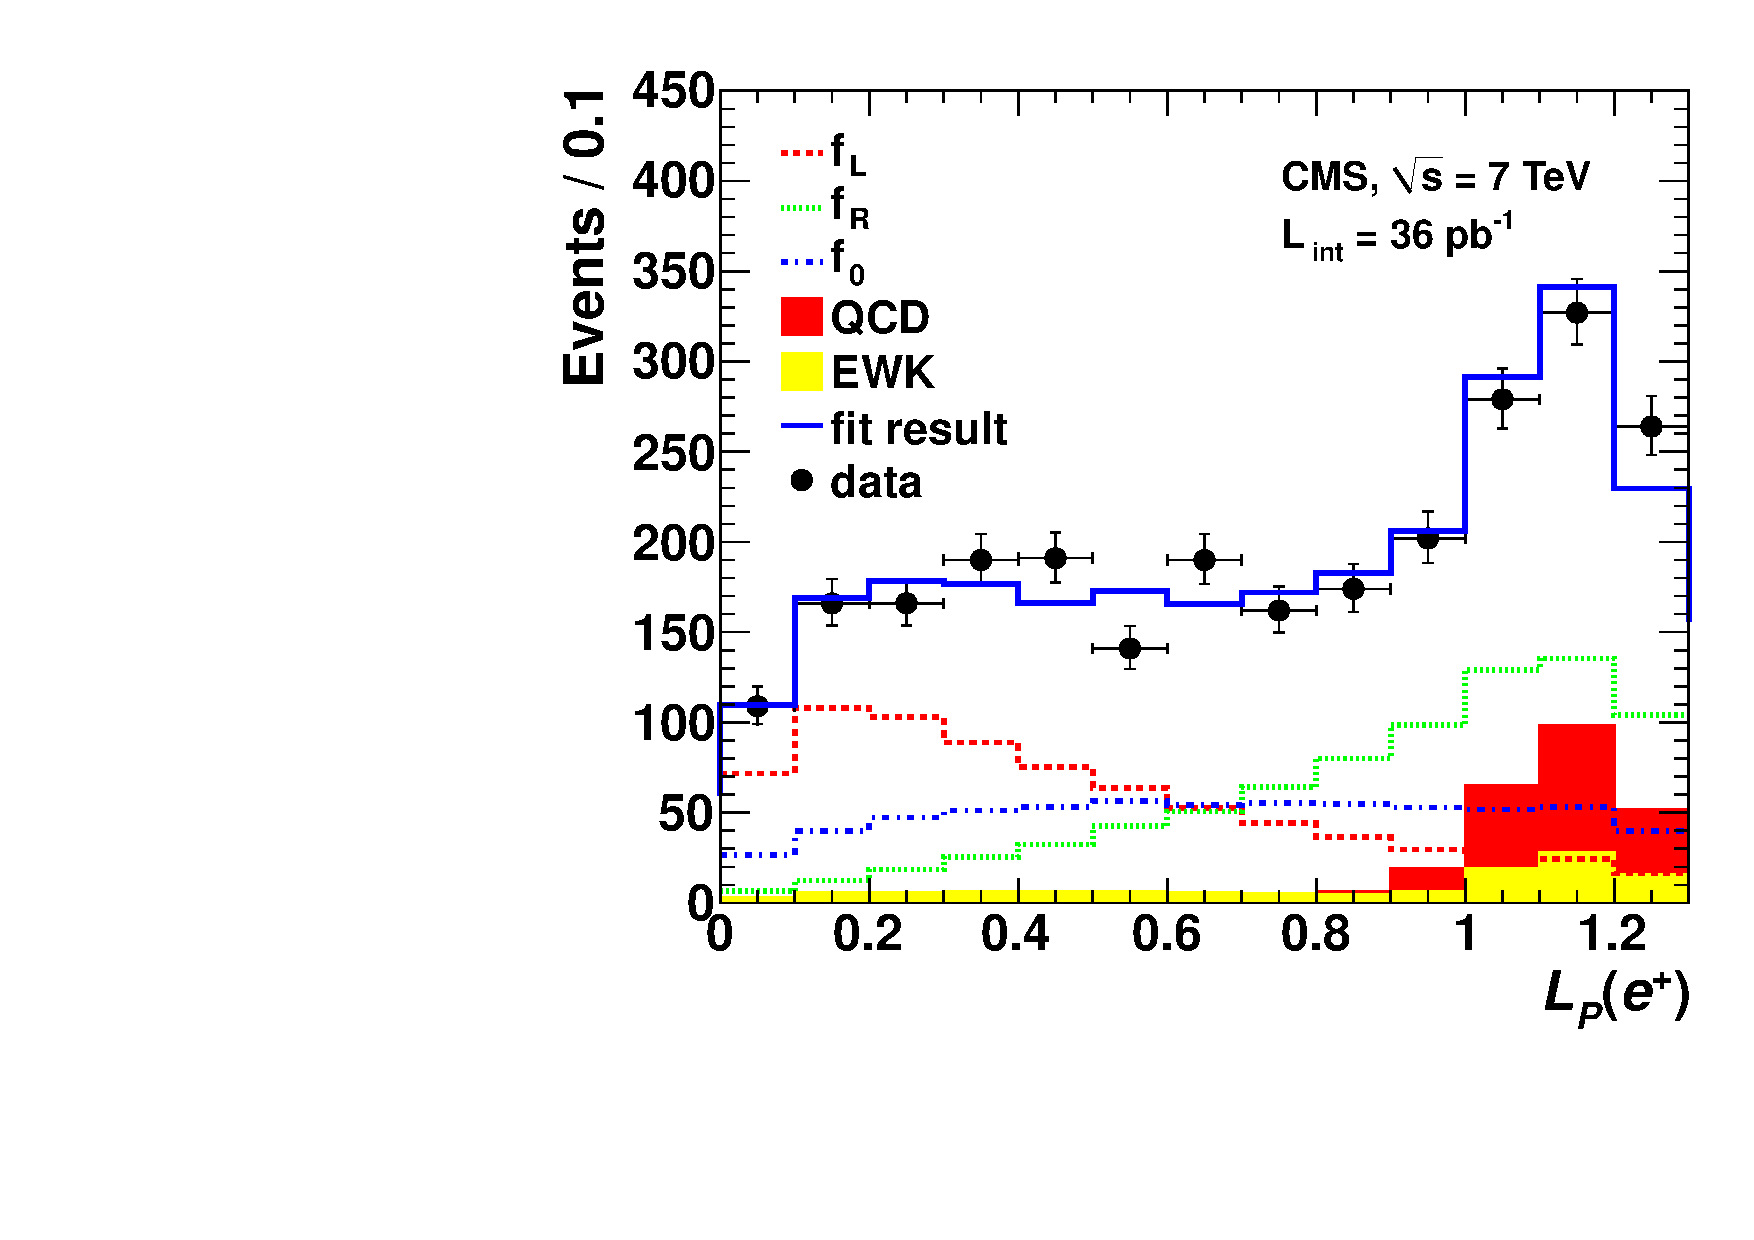
\includegraphics[width=0.45\textwidth]{fig/electron_MC_WHelicityFramePlots_PlusICVar}}\\
\subfloat[]{\label{fig:wpol_fit_mu_plus}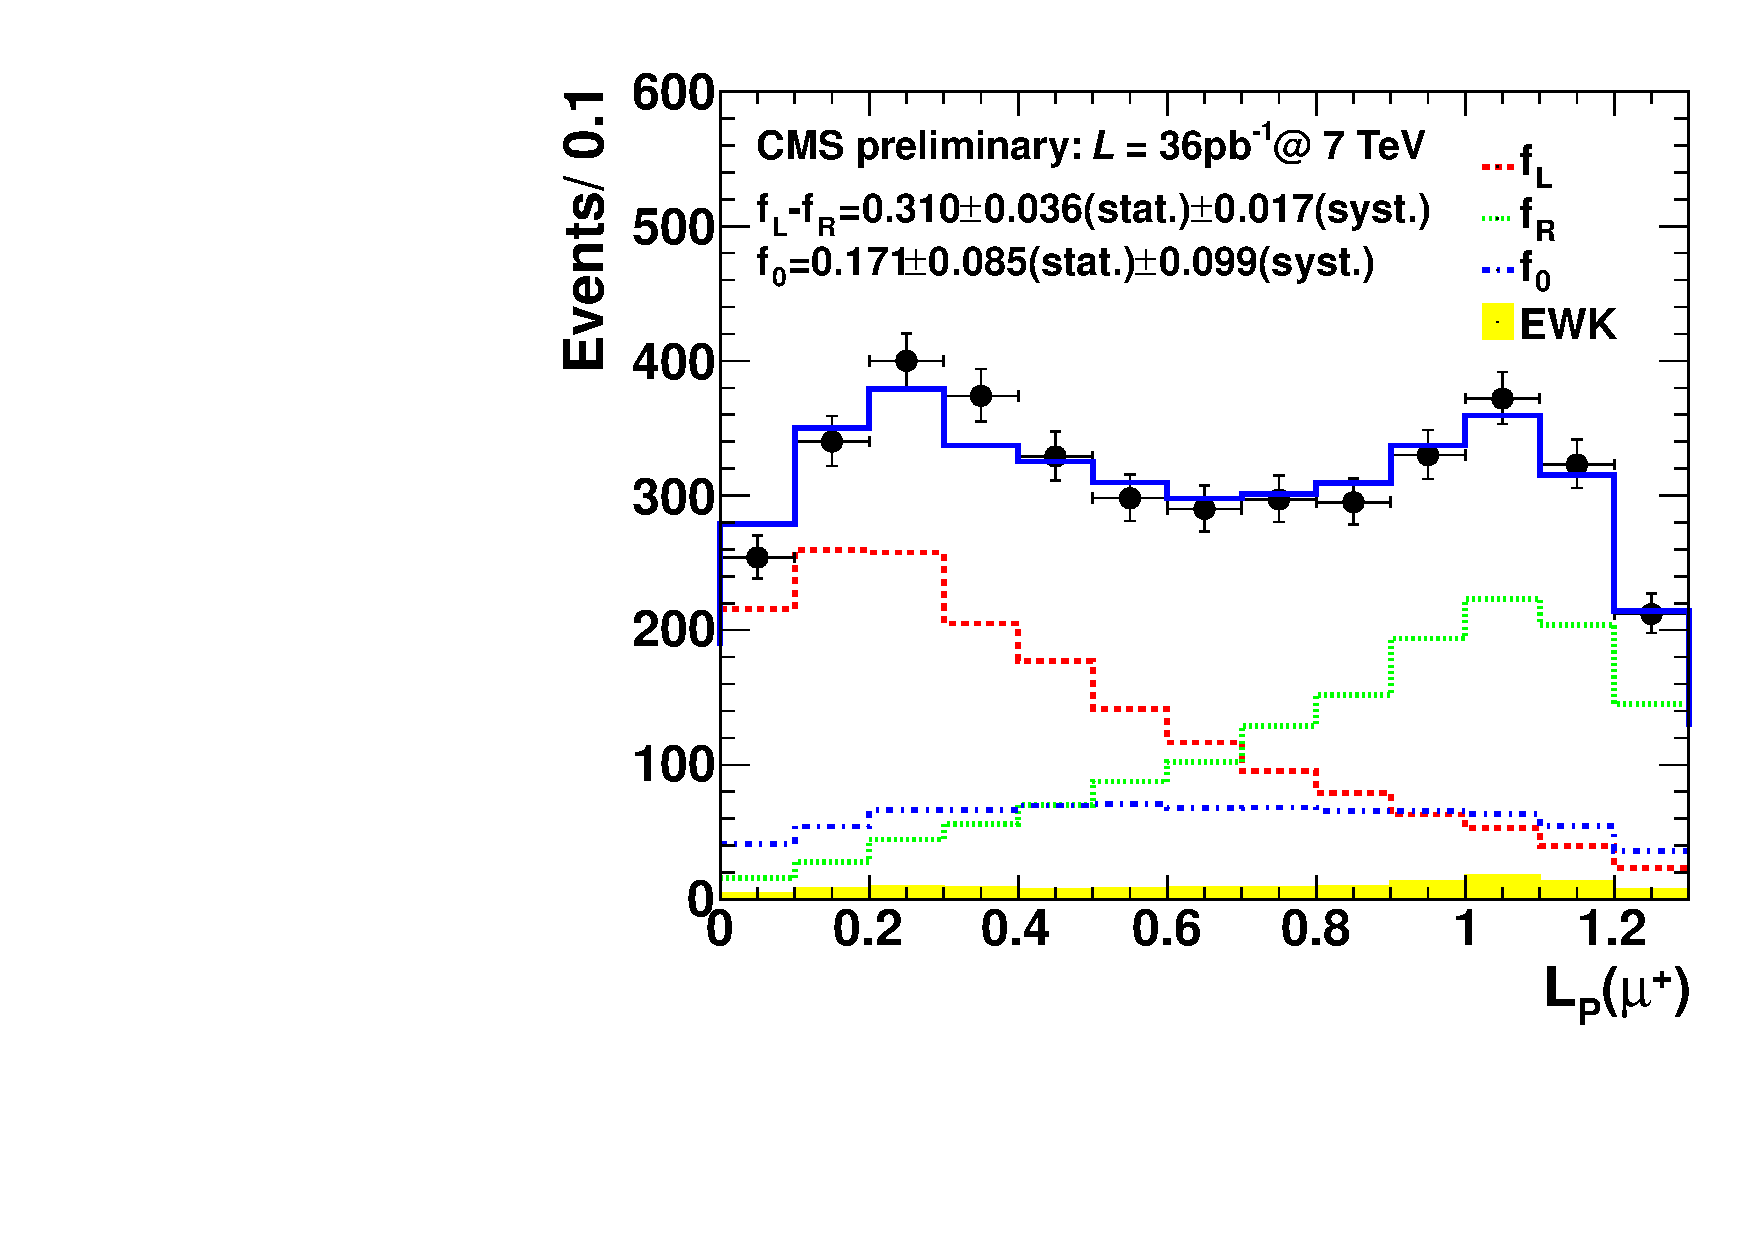
\includegraphics[width=0.45\textwidth]{fig/MC_WHelicityFramePlots_PlusICVar}}\quad
\subfloat[]{\label{fig:wpol_fit_mu_minus}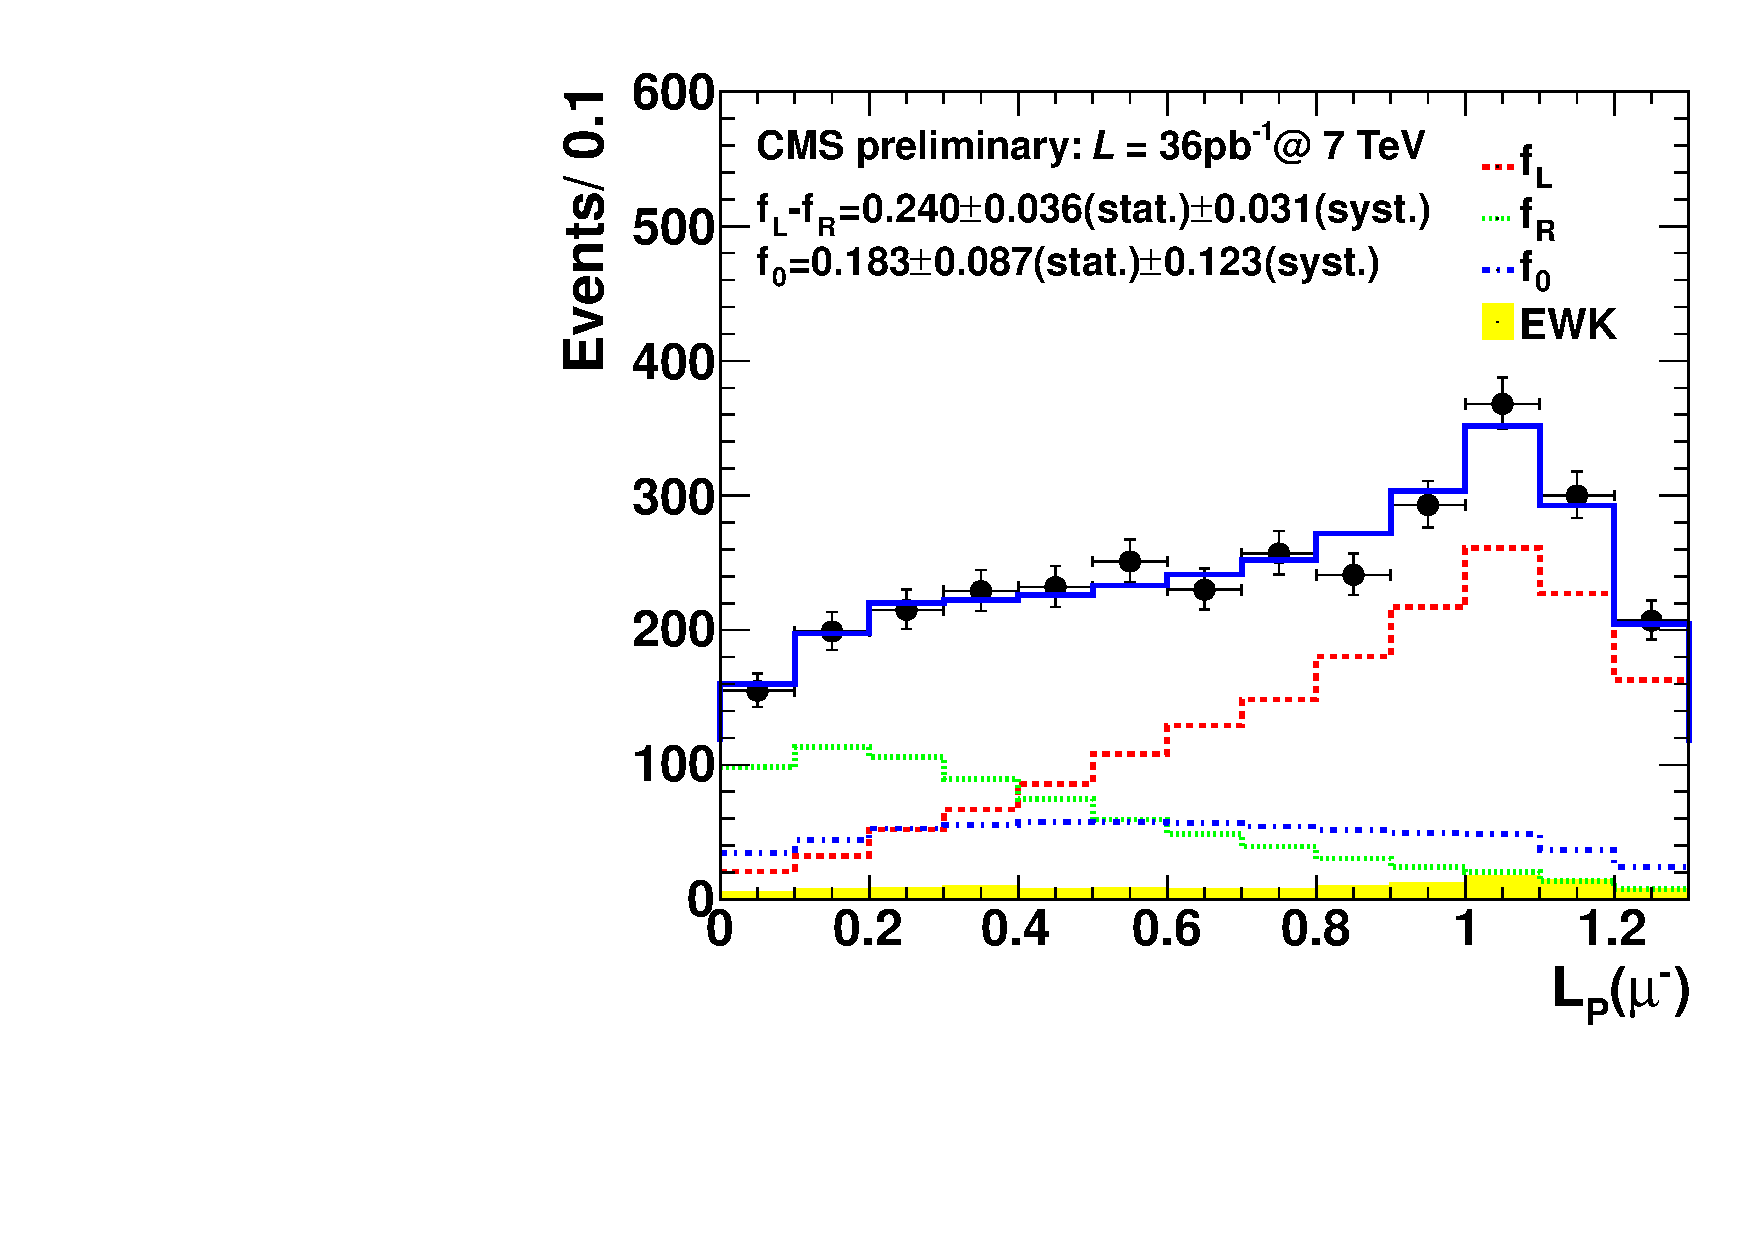
\includegraphics[width=0.45\textwidth]{fig/MC_WHelicityFramePlots_MinusICVar}}
\caption{Fit results}
\label{fig:wpol_fit_results}
\end{figure}


\begin{figure}
\centering
\subfloat[]{\label{fig:wpol_contour_ele_plus}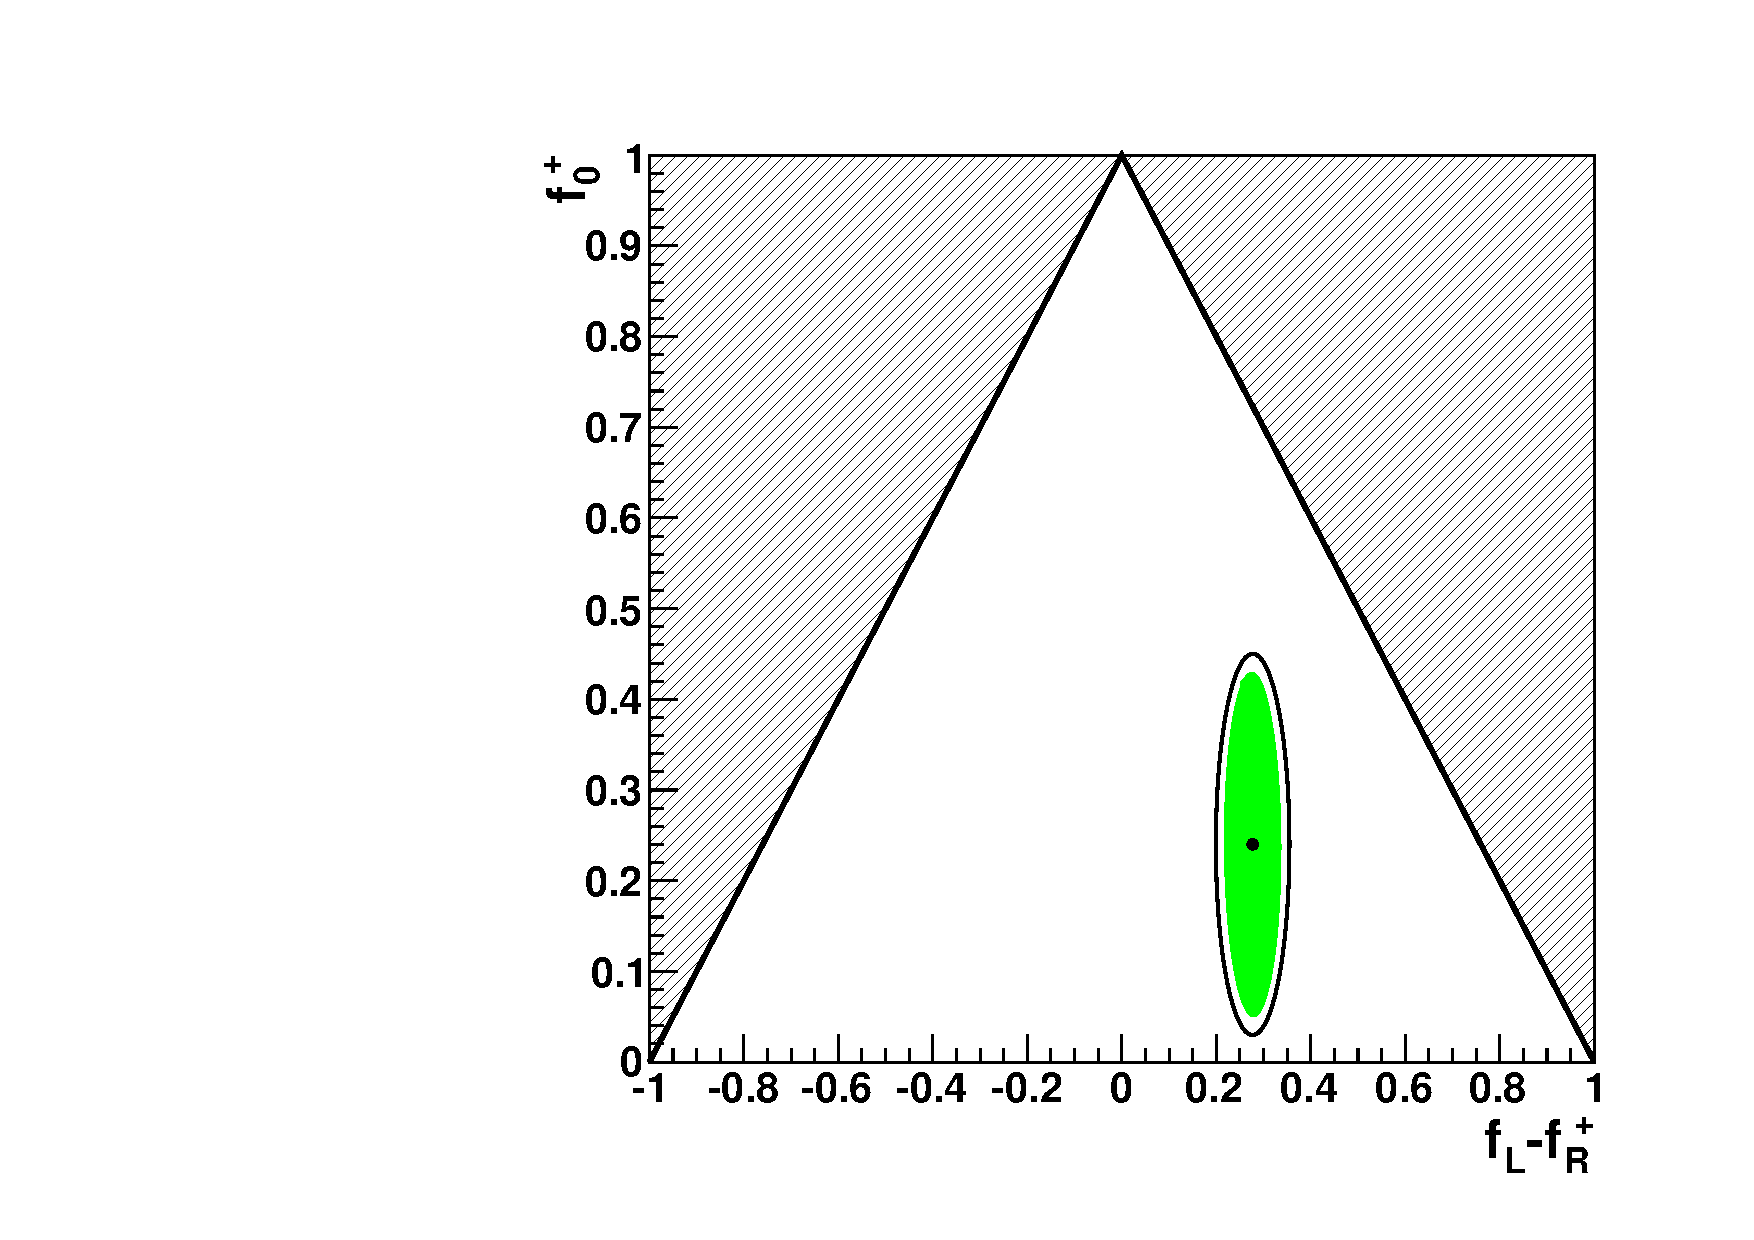
\includegraphics[width=0.45\textwidth]{fig/electron_contour_plus}}\quad
\subfloat[]{\label{fig:wpol_contour_ele_minus}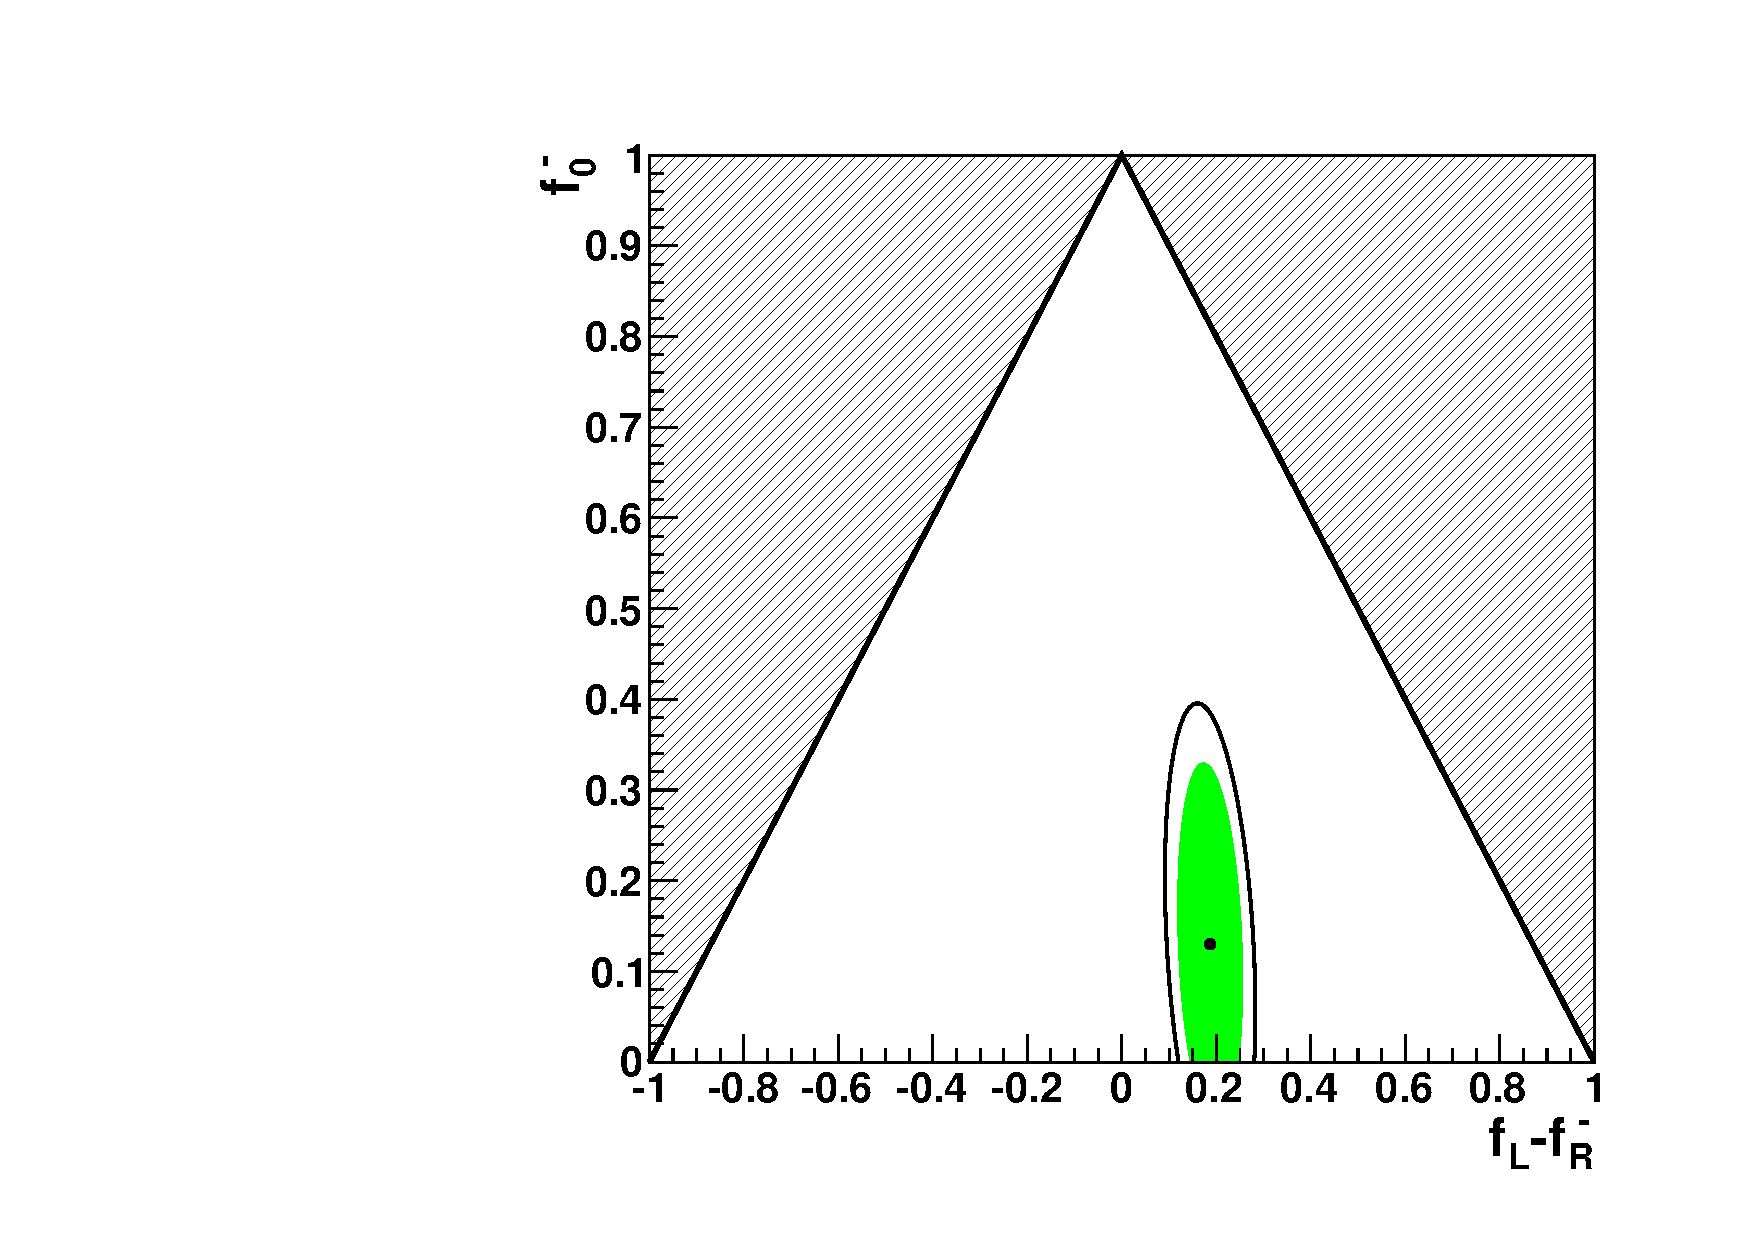
\includegraphics[width=0.45\textwidth]{fig/electron_contour_minus}}
\caption{Contours}
\label{fig:wpol_contour_ele}
\end{figure}

\begin{figure}
\centering
\subfloat[]{\label{fig:wpol_contour_mu_plus}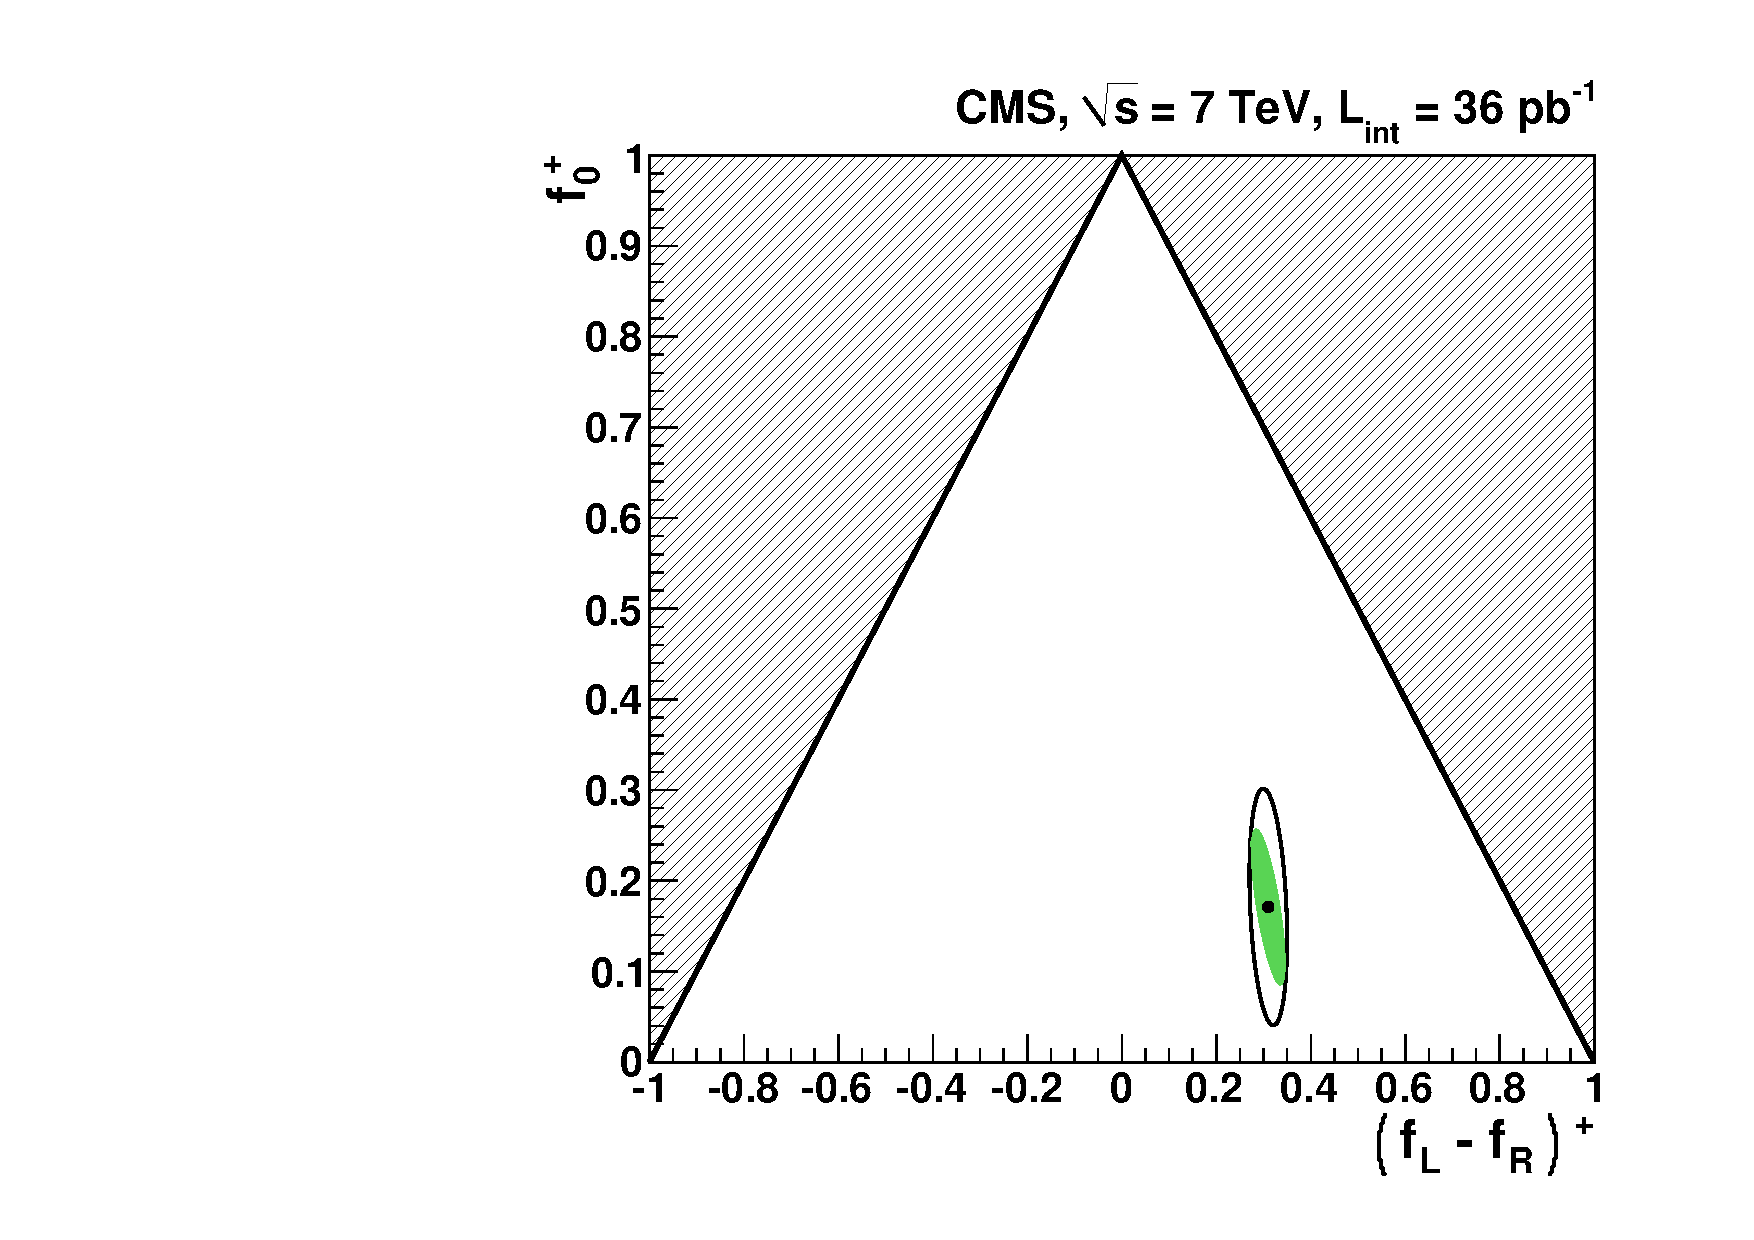
\includegraphics[width=0.45\textwidth]{fig/muon_contour_plus}}\quad
\subfloat[]{\label{fig:wpol_contour_mu_minus}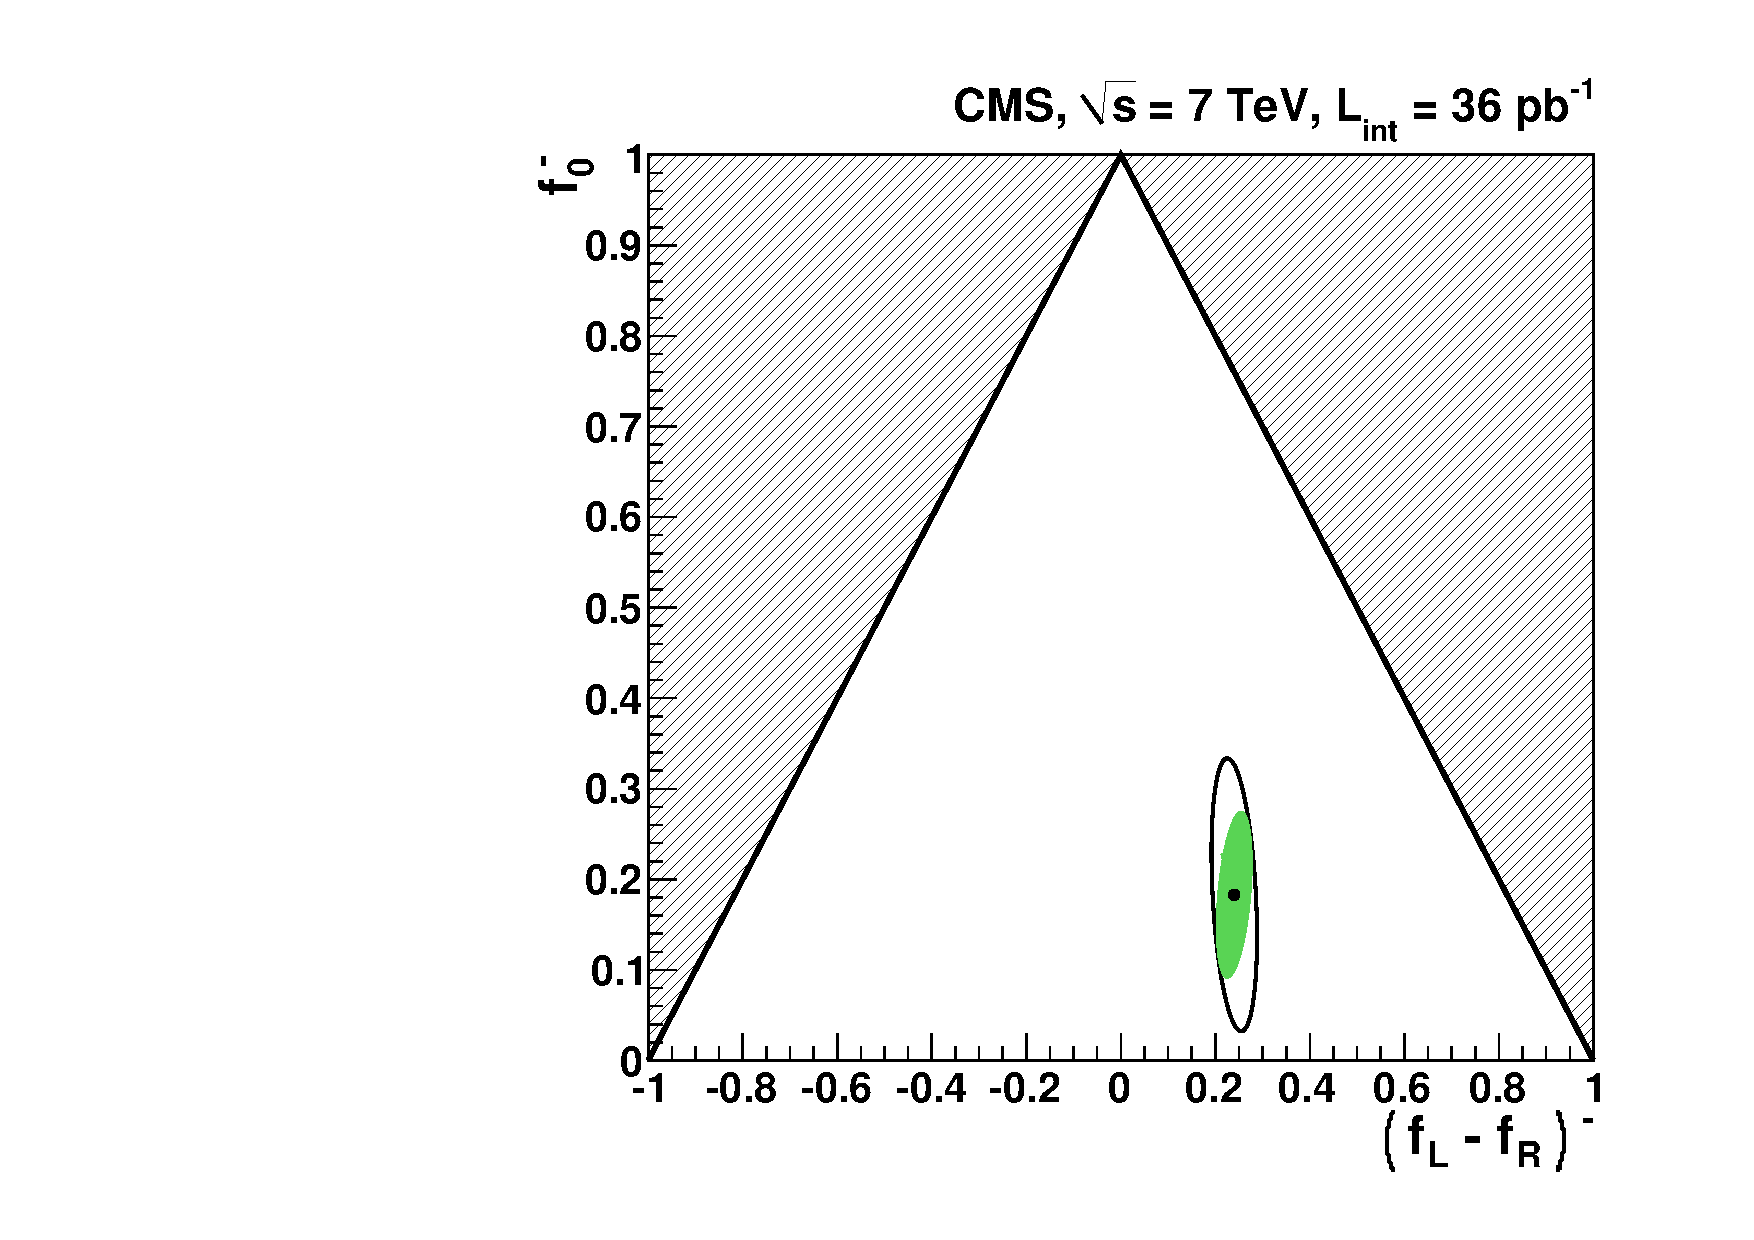
\includegraphics[width=0.45\textwidth]{fig/muon_contour_minus}}
\caption{Contours}
\label{fig:wpol_contour_mu}
\end{figure}

Two combined fits have also been performed across both lepton flavours, one for
each lepton charge. The error contours are shown in
Figure~\ref{fig:wpol_contour_comb}.
\begin{figure}
\centering
\subfloat[]{\label{fig:wpol_contour_comb_plus}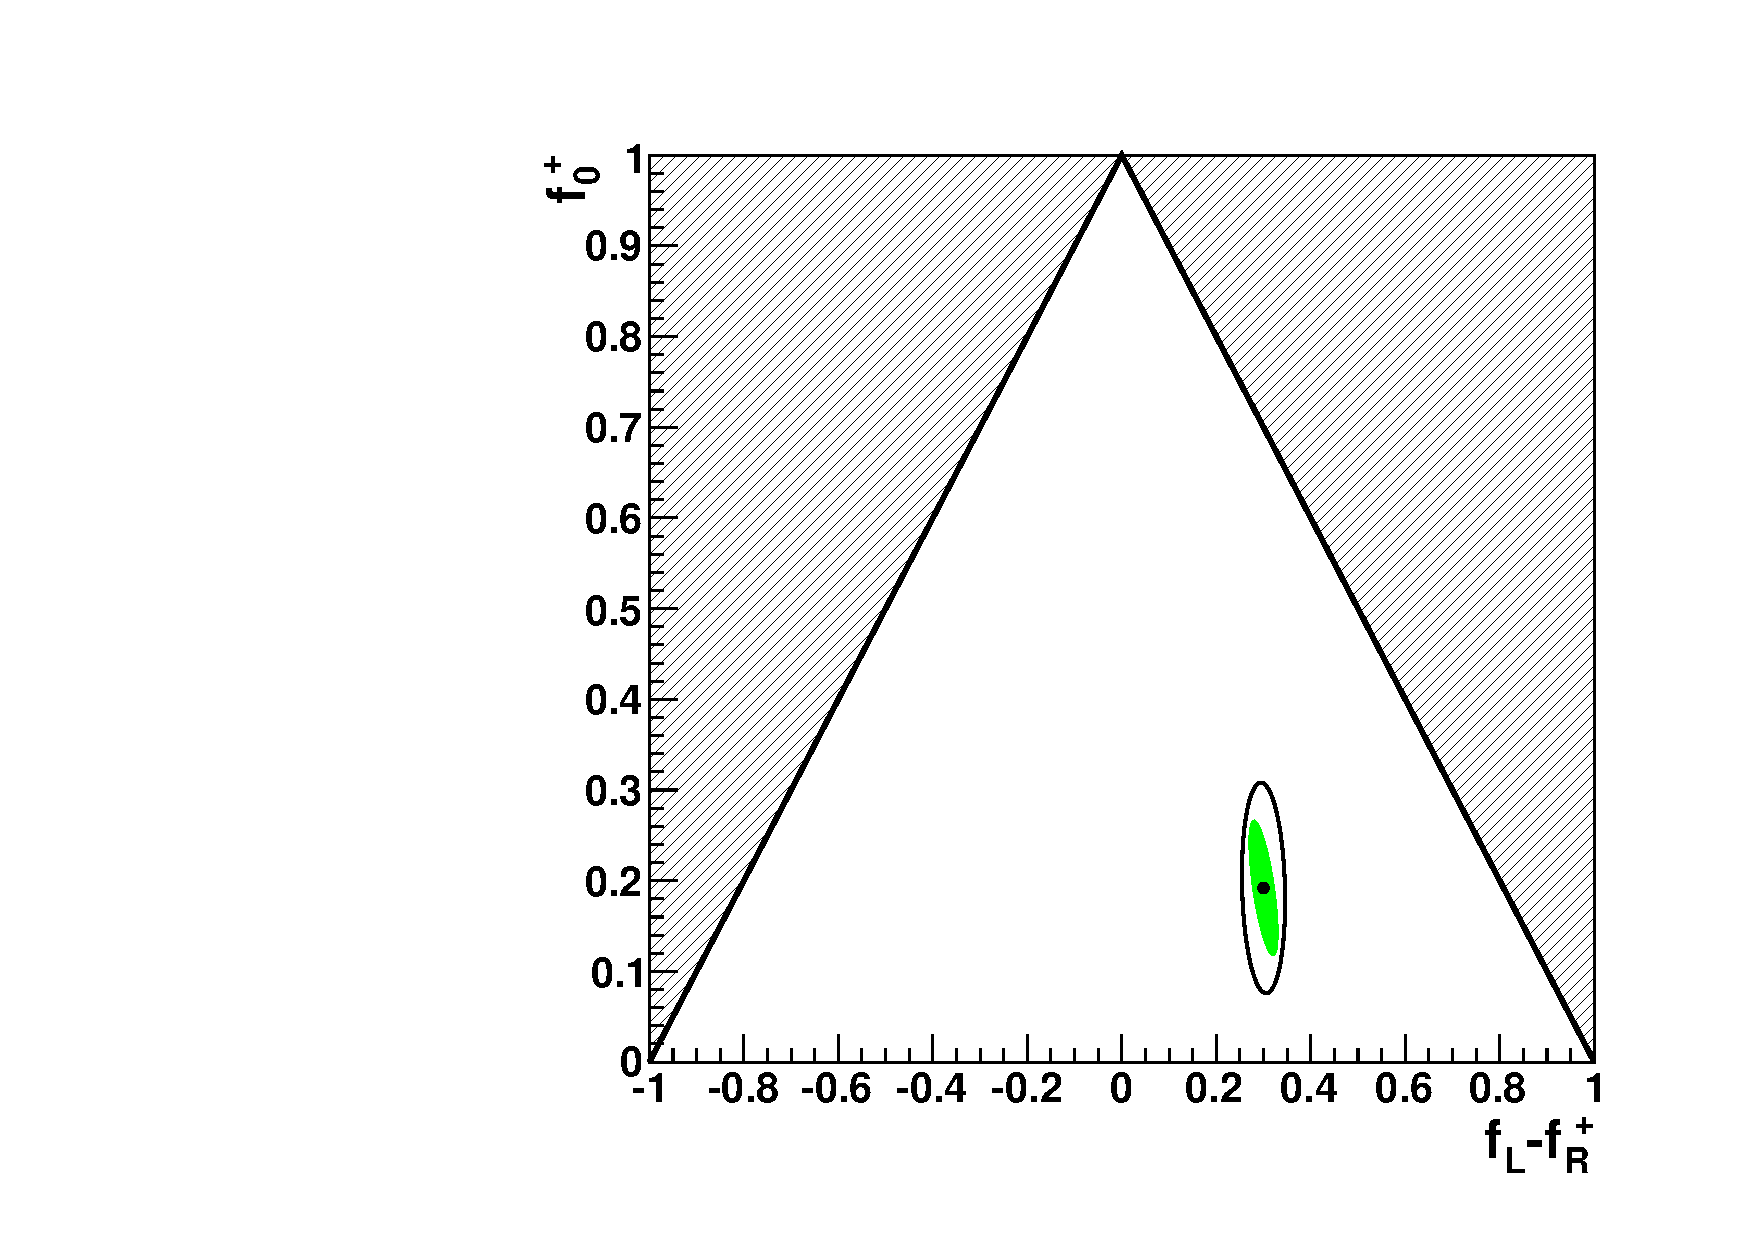
\includegraphics[width=0.45\textwidth]{fig/combined_contour_plus}}\quad
\subfloat[]{\label{fig:wpol_contour_comb_minus}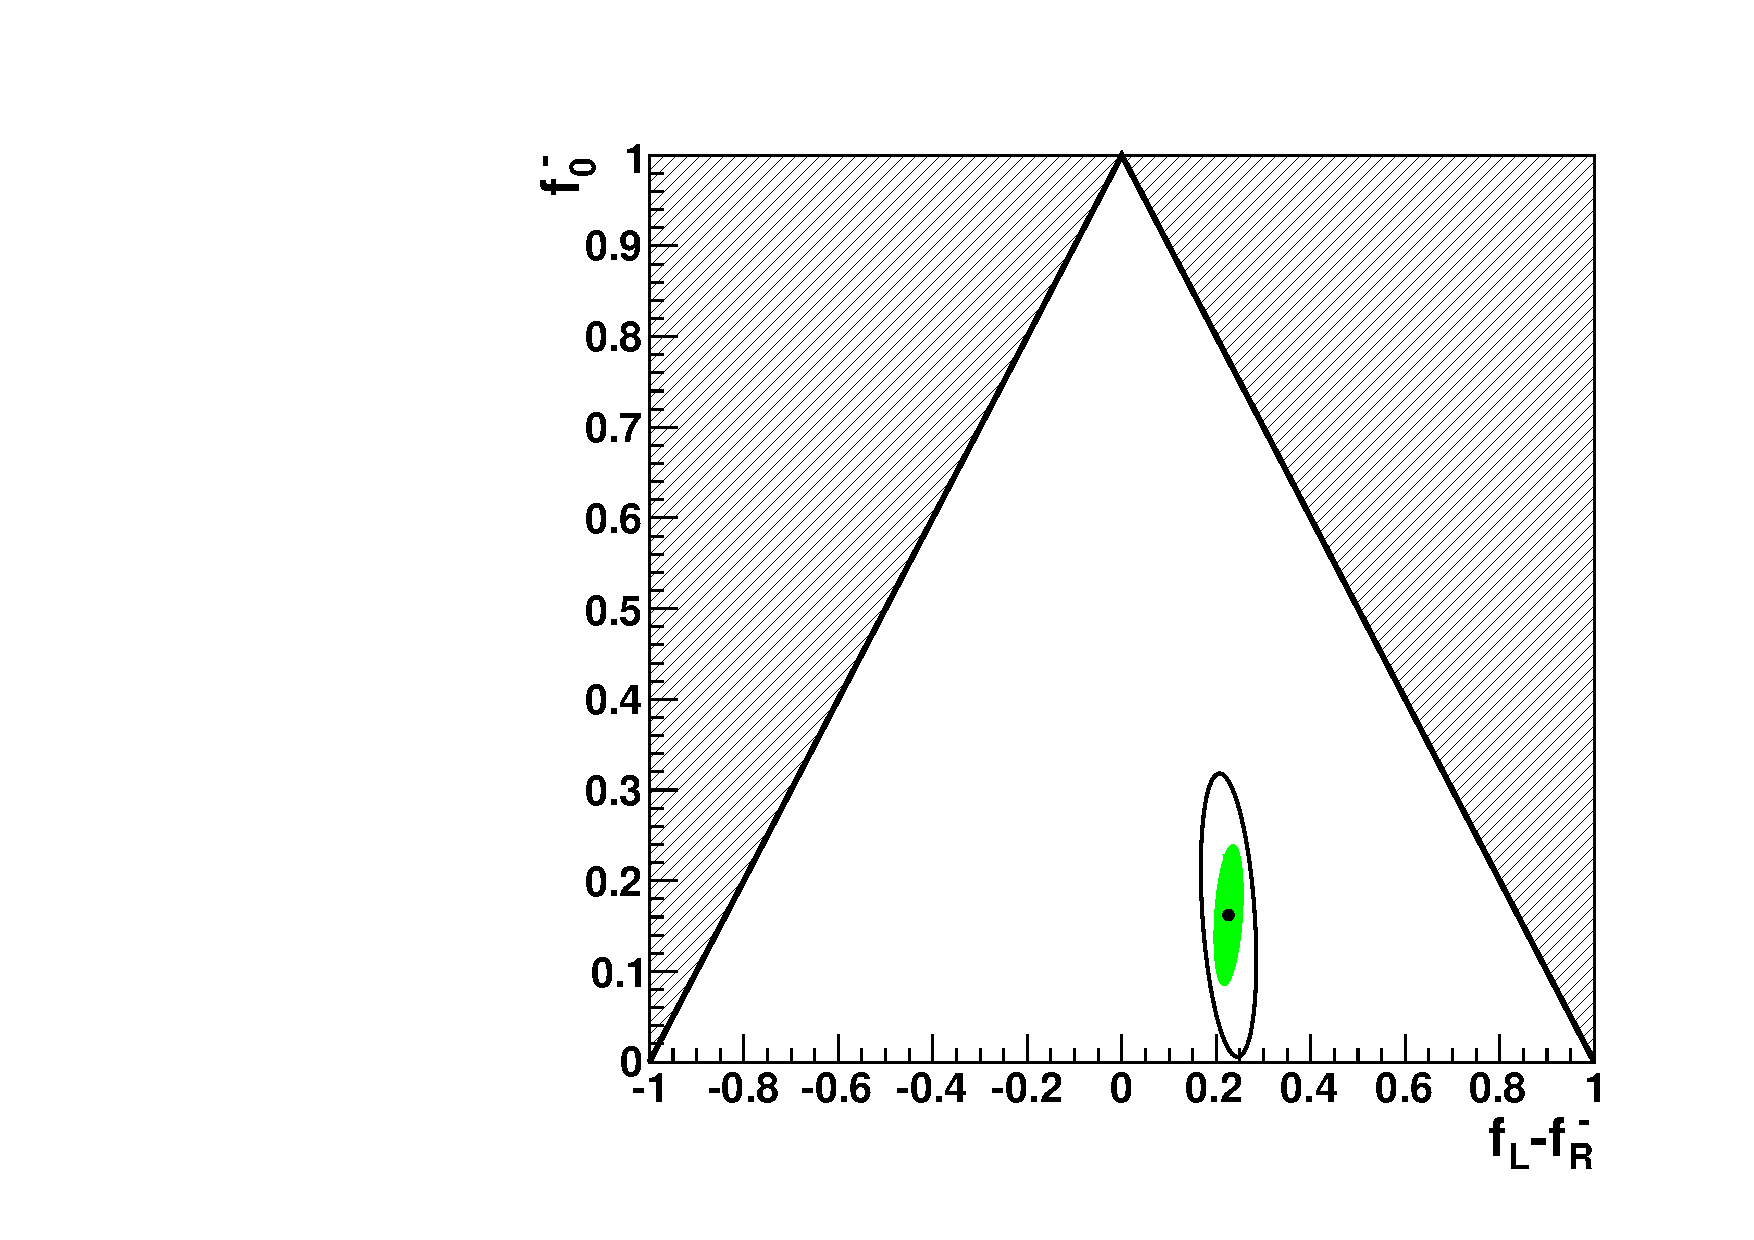
\includegraphics[width=0.45\textwidth]{fig/combined_contour_minus}}
\caption{Contours}
\label{fig:wpol_contour_comb}
\end{figure}

The results of each fit are presented in Table~\ref{tbl:wpol_fitresults} along
with statistical and systematic errors. Also shown are the global correlation in
each case and the \chisq measure of the goodness-of-fit.

\ctable[
cap=Summary of fit results in the \PW polarisation measurement,
caption={A summary of the fit results for \fLmfR and \f0 in the muon, electron
and combined channels. The statistical and systematic uncertainties are given
for each measurement. The global correlation is also shown for each case as well
as the $\chi^2$/ndof measure of the goodness-of-fit.},
label=tbl:wpol_fitresults,
mincapwidth=0.7\textwidth,
%doinside=\scriptsize,
pos=h!
]{ c c }{
}{\FL
                              &  Data Fit Result                                                   \ML
 $\mu: \fLmfR^{-}$   & $0.240 \pm 0.036$ (stat.) $\pm0.031$ (syst.)   \NN
 $\mu: \f0^{-}$             & $0.183 \pm 0.087 \pm 0.123$                             \NN
 Correlation                  & 0.395  (stat.)                                                  \NN
 $\chi^2$/ndof  (stat)        & $0.767$                                                                        \ML
 $\mu: \fLmfR^{+}$     & $0.310 \pm 0.036 \pm 0.017$                                              \NN
 $\mu: \f0^{+}$             & $0.171 \pm 0.085 \pm 0.099$                                              \NN
 Correlation                  & -0.721  (stat.)                                                            \NN
 $\chi^2$/ndof  (stat)        & $0.967$                                                                       \ML
 $e: \fLmfR^{-}$     & $0.187 \pm 0.069$ (stat.)  $\pm 0.066$ (syst.)                          \NN
 $e: \f0^{-}$               & $0.130 \pm 0.200$ $\pm 0.174$                                           \NN
 Correlation (stat)           & -0.204    (stat.)                                                         \NN
 $\chi^2$/ndof  (stat)        & $0.872$                                                                      \ML
 $e: \fLmfR^{+}$       & $0.277 \pm 0.060$ $\pm 0.050$                                                    \NN
 $e: \f0^{+}$               & $0.24 \pm 0.190$ $\pm 0.090$                                                       \NN
 Correlation (stat)           & -0.295 (stat.)                                                                       \NN
 $\chi^2$/ndof (stat)       & $2.239$                                                                         \ML
 comb: $\fLmfR^{-}$  &  $0.226 \pm 0.031$ (stat.) $\pm 0.050$ (syst.)                            \NN
 comb: $\f0^{-}$            &  $0.162 \pm 0.078$ (stat.) $\pm 0.136$ (syst.)                              \NN
 Correlation (stat)           &  0.304 (stat.)                                                                \ML
 comb: $\fLmfR^{+}$    &  $0.300 \pm 0.031$ (stat.) $\pm 0.034$ (syst.)                                \NN
 comb: $\f0^{+}$            &  $0.192 \pm 0.075$ (stat.) $\pm 0.089$ (syst.)                                 \NN
 Correlation (stat)           &  -0.660  (stat.)                                                                 \LL
}
\ctable[
  cap=Summary of the \PW polarisation fit results for the \ac{QCD} background,
  caption=A summary of the fit results for the \ac{QCD} background component in
  the electron-only and combined fits. \fQCD is the fraction of QCD events
  determined from the fit. $N_{QCD}$ is the estimated number of QCD events. The
  correlation with the polarisation fit parameters is also given.,
  label=tbl:fqcd_fit_results,
  doinside=\footnotesize
]{ c c c c c}{
}{\FL
                & $f_{QCD}$         & $N_{QCD}$          & correlation ($(f_{L}-f_{R})$,$f_{QCD}$) &  correlation ($f_{0}$,$f_{QCD}$)  \ML
  $e^-$         & $0.094 \pm 0.056$ & $221.3 \pm 131.8$  &  -0.540 & 0.840  \NN
  $e^+$         & $0.098 \pm 0.042$ & $284.5 \pm 121.9$  &  0.198 & 0.808  \NN
  $(e+\mu)^{-}$ & $0.089 \pm 0.025$ & $209.5 \pm 58.9$   &  -0.172 & 0.493   \NN
  $(e+\mu)^{+}$ & $0.094 \pm 0.020$ & $272.9 \pm 58.1$   &   0.018 & 0.476    \LL
}

\ctable[
caption=Comparison of the CMS \PW polarisation measurement with theoretical
results from \cite{berger_left_handed_w}. The theoretical predictions are at
\ac{NLO}\, \ac{ME+PS} and \ac{LO}. The difference between the \ac{NLO} may be
taken as an approximate uncertainty,
pos=h,
label=tbl:wpol_theory_comparison,
%doinside=\scriptsize
]{lcccc}{
}{\FL
      & $f_0^-$                   & $(f_L -f_R)^-$            & $f_0^+$                   & $(f_L-f_R)^+$ \ML
CMS   & 0.162$\pm$0.078$\pm$0.136 & 0.226$\pm$0.031$\pm$0.050 & 0.192$\pm$0.075$\pm$0.089 & 0.300$\pm$0.031$\pm$0.034 \NN
NLO   & 0.193                     & 0.248                     & 0.200                     & 0.308             \NN
ME+PS & 0.179                     & 0.222                     & 0.187                     & 0.283 \NN
LO    & 0.190                     & 0.235                     & 0.198                     & 0.309 \LL
}

\section{Conclusions}
As has been seen, the transverse polarisation of the \PW boson has been measured
at \ac{CMS} using \unit{36}{\invpb} of data from the 2010 run of the
\ac{LHC}. The parameter, \fLmfR has been measured independently in the muon and
electron channels for leptons of identical charge and for \PW boson with
transverse momentum greater than \unit{50}{\GeV}. In addition, a combined
measurement has been obtained via a simultaneous fit to both channels, again
separated by lepton charge. The most precise measurement is provided by the muon
channel alone. The dominant left-handed polarisation effect described in
Section~\ref{sec:polarisation} is established with a significance of 7.8 and 5.1
$\sigma$ for \PWp and \PWm respectively.

Whilst the primary goal of the measurement was to confirm the transverse
polarisation effect, the longitudinal polarisation fraction has also been
measured, albeit with less sensitivity.

After publication of this result \cite{cms_wpol_paper}, a set of theoretical
predictions were published \cite{berger_left_handed_w}. The Blackhat Monte Carlo
generator was used to compare like-for-like with this measurement. This
comparison is shown in Table~\ref{tbl:wpol_theory_comparison}. It can be seen
that this measurement agrees well with the theoretical expectations.

%%% Local Variables:
%%% mode: latex
%%% TeX-master: "../thesis"
%%% End:
